% Created by tikzDevice version 0.9 on 2016-01-09 17:06:54
% !TEX encoding = UTF-8 Unicode
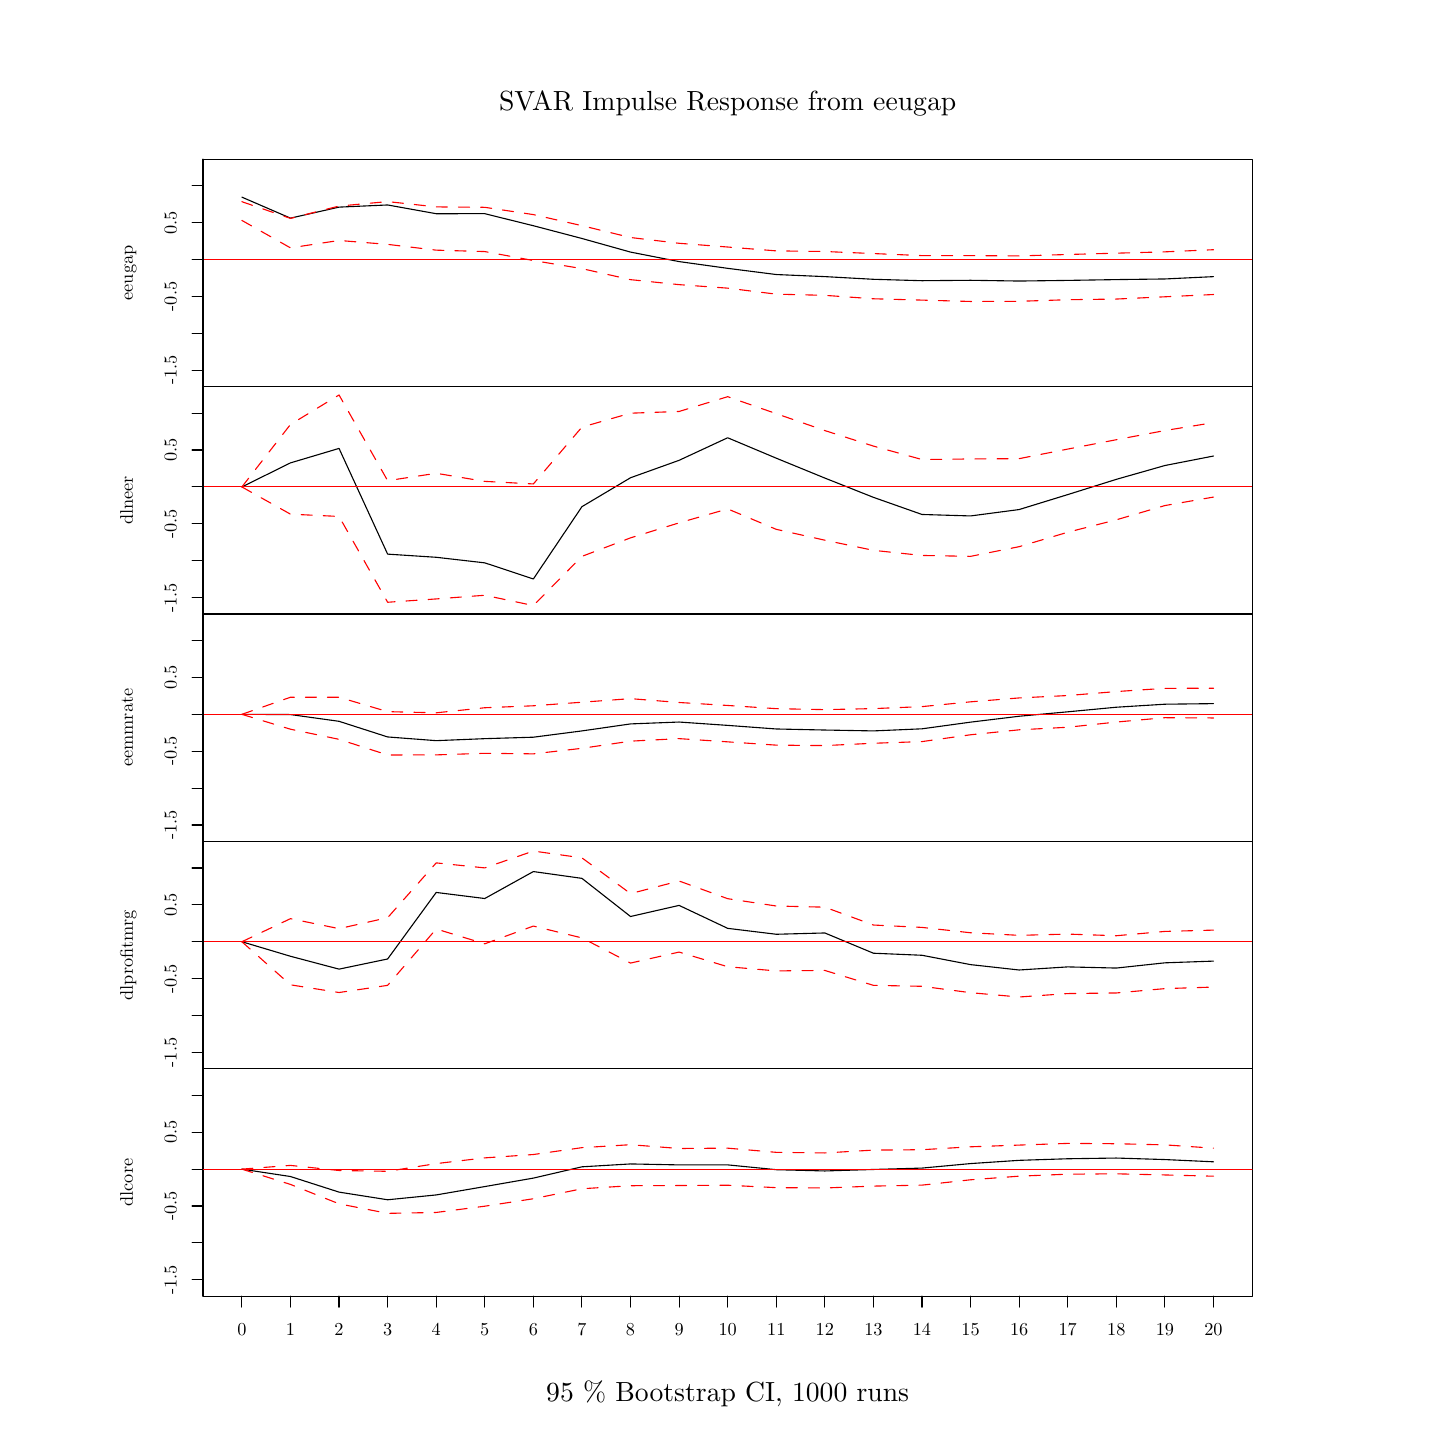
\begin{tikzpicture}[x=1pt,y=1pt]
\definecolor{fillColor}{RGB}{255,255,255}
\path[use as bounding box,fill=fillColor,fill opacity=0.00] (0,0) rectangle (505.89,505.89);
\begin{scope}
\path[clip] ( 63.36,376.20) rectangle (442.53,458.37);
\definecolor{drawColor}{RGB}{0,0,0}

\path[draw=drawColor,line width= 0.4pt,line join=round,line cap=round] ( 77.40,444.65) --
	( 94.96,437.06) --
	(112.51,441.04) --
	(130.07,441.82) --
	(147.62,438.66) --
	(165.17,438.67) --
	(182.73,434.32) --
	(200.28,429.71) --
	(217.84,424.79) --
	(235.39,421.36) --
	(252.94,418.92) --
	(270.50,416.68) --
	(288.05,415.93) --
	(305.61,414.96) --
	(323.16,414.45) --
	(340.72,414.60) --
	(358.27,414.33) --
	(375.82,414.56) --
	(393.38,414.85) --
	(410.93,415.08) --
	(428.49,415.92);
\end{scope}
\begin{scope}
\path[clip] ( 31.68,376.20) rectangle (474.21,458.37);
\definecolor{drawColor}{RGB}{0,0,0}

\node[text=drawColor,anchor=base,inner sep=0pt, outer sep=0pt, scale=  0.66] at (252.94,346.10) {xy{\$}x};

\node[text=drawColor,rotate= 90.00,anchor=base,inner sep=0pt, outer sep=0pt, scale=  0.66] at ( 38.02,417.29) {eeugap};
\end{scope}
\begin{scope}
\path[clip] (  0.00,  0.00) rectangle (505.89,505.89);
\definecolor{drawColor}{RGB}{0,0,0}

\path[draw=drawColor,line width= 0.4pt,line join=round,line cap=round] ( 63.36,382.11) -- ( 63.36,458.37);

\path[draw=drawColor,line width= 0.4pt,line join=round,line cap=round] ( 63.36,382.11) -- ( 59.40,382.11);

\path[draw=drawColor,line width= 0.4pt,line join=round,line cap=round] ( 63.36,395.44) -- ( 59.40,395.44);

\path[draw=drawColor,line width= 0.4pt,line join=round,line cap=round] ( 63.36,408.77) -- ( 59.40,408.77);

\path[draw=drawColor,line width= 0.4pt,line join=round,line cap=round] ( 63.36,422.10) -- ( 59.40,422.10);

\path[draw=drawColor,line width= 0.4pt,line join=round,line cap=round] ( 63.36,435.43) -- ( 59.40,435.43);

\path[draw=drawColor,line width= 0.4pt,line join=round,line cap=round] ( 63.36,448.76) -- ( 59.40,448.76);

\node[text=drawColor,rotate= 90.00,anchor=base,inner sep=0pt, outer sep=0pt, scale=  0.66] at ( 53.86,382.11) {-1.5};

\node[text=drawColor,rotate= 90.00,anchor=base,inner sep=0pt, outer sep=0pt, scale=  0.66] at ( 53.86,408.77) {-0.5};

\node[text=drawColor,rotate= 90.00,anchor=base,inner sep=0pt, outer sep=0pt, scale=  0.66] at ( 53.86,435.43) {0.5};
\end{scope}
\begin{scope}
\path[clip] ( 63.36,376.20) rectangle (442.53,458.37);
\definecolor{drawColor}{RGB}{255,0,0}

\path[draw=drawColor,line width= 0.4pt,line join=round,line cap=round] ( 63.36,422.10) -- (442.53,422.10);

\path[draw=drawColor,line width= 0.4pt,dash pattern=on 4pt off 4pt ,line join=round,line cap=round] ( 77.40,443.00) --
	( 94.96,436.97) --
	(112.51,441.42) --
	(130.07,443.04) --
	(147.62,441.12) --
	(165.17,440.97) --
	(182.73,438.34) --
	(200.28,434.34) --
	(217.84,430.06) --
	(235.39,427.97) --
	(252.94,426.62) --
	(270.50,425.23) --
	(288.05,425.00) --
	(305.61,424.26) --
	(323.16,423.52) --
	(340.72,423.50) --
	(358.27,423.41) --
	(375.82,423.92) --
	(393.38,424.40) --
	(410.93,424.88) --
	(428.49,425.65);

\path[draw=drawColor,line width= 0.4pt,dash pattern=on 4pt off 4pt ,line join=round,line cap=round] ( 77.40,436.24) --
	( 94.96,426.32) --
	(112.51,428.99) --
	(130.07,427.58) --
	(147.62,425.49) --
	(165.17,424.98) --
	(182.73,421.74) --
	(200.28,418.82) --
	(217.84,414.83) --
	(235.39,413.03) --
	(252.94,411.76) --
	(270.50,409.59) --
	(288.05,409.16) --
	(305.61,407.92) --
	(323.16,407.44) --
	(340.72,406.95) --
	(358.27,407.01) --
	(375.82,407.58) --
	(393.38,407.82) --
	(410.93,408.64) --
	(428.49,409.46);
\end{scope}
\begin{scope}
\path[clip] (  0.00,  0.00) rectangle (505.89,505.89);
\definecolor{drawColor}{RGB}{0,0,0}

\path[draw=drawColor,line width= 0.4pt,line join=round,line cap=round] ( 63.36,376.20) --
	(442.53,376.20) --
	(442.53,458.37) --
	( 63.36,458.37) --
	( 63.36,376.20);
\end{scope}
\begin{scope}
\path[clip] ( 63.36,294.03) rectangle (442.53,376.20);
\definecolor{drawColor}{RGB}{0,0,0}

\path[draw=drawColor,line width= 0.4pt,line join=round,line cap=round] ( 77.40,339.93) --
	( 94.96,348.62) --
	(112.51,353.85) --
	(130.07,315.65) --
	(147.62,314.51) --
	(165.17,312.50) --
	(182.73,306.68) --
	(200.28,332.80) --
	(217.84,343.25) --
	(235.39,349.55) --
	(252.94,357.70) --
	(270.50,350.32) --
	(288.05,343.14) --
	(305.61,336.17) --
	(323.16,329.98) --
	(340.72,329.45) --
	(358.27,331.76) --
	(375.82,337.16) --
	(393.38,342.67) --
	(410.93,347.67) --
	(428.49,351.10);
\end{scope}
\begin{scope}
\path[clip] ( 31.68,294.03) rectangle (474.21,376.20);
\definecolor{drawColor}{RGB}{0,0,0}

\node[text=drawColor,anchor=base,inner sep=0pt, outer sep=0pt, scale=  0.66] at (252.94,263.93) {xy{\$}x};

\node[text=drawColor,rotate= 90.00,anchor=base,inner sep=0pt, outer sep=0pt, scale=  0.66] at ( 38.02,335.12) {dlneer};
\end{scope}
\begin{scope}
\path[clip] (  0.00,  0.00) rectangle (505.89,505.89);
\definecolor{drawColor}{RGB}{0,0,0}

\path[draw=drawColor,line width= 0.4pt,line join=round,line cap=round] ( 63.36,299.94) -- ( 63.36,376.20);

\path[draw=drawColor,line width= 0.4pt,line join=round,line cap=round] ( 63.36,299.94) -- ( 59.40,299.94);

\path[draw=drawColor,line width= 0.4pt,line join=round,line cap=round] ( 63.36,313.27) -- ( 59.40,313.27);

\path[draw=drawColor,line width= 0.4pt,line join=round,line cap=round] ( 63.36,326.60) -- ( 59.40,326.60);

\path[draw=drawColor,line width= 0.4pt,line join=round,line cap=round] ( 63.36,339.93) -- ( 59.40,339.93);

\path[draw=drawColor,line width= 0.4pt,line join=round,line cap=round] ( 63.36,353.26) -- ( 59.40,353.26);

\path[draw=drawColor,line width= 0.4pt,line join=round,line cap=round] ( 63.36,366.59) -- ( 59.40,366.59);

\node[text=drawColor,rotate= 90.00,anchor=base,inner sep=0pt, outer sep=0pt, scale=  0.66] at ( 53.86,299.94) {-1.5};

\node[text=drawColor,rotate= 90.00,anchor=base,inner sep=0pt, outer sep=0pt, scale=  0.66] at ( 53.86,326.60) {-0.5};

\node[text=drawColor,rotate= 90.00,anchor=base,inner sep=0pt, outer sep=0pt, scale=  0.66] at ( 53.86,353.26) {0.5};
\end{scope}
\begin{scope}
\path[clip] ( 63.36,294.03) rectangle (442.53,376.20);
\definecolor{drawColor}{RGB}{255,0,0}

\path[draw=drawColor,line width= 0.4pt,line join=round,line cap=round] ( 63.36,339.93) -- (442.53,339.93);

\path[draw=drawColor,line width= 0.4pt,dash pattern=on 4pt off 4pt ,line join=round,line cap=round] ( 77.40,339.93) --
	( 94.96,362.51) --
	(112.51,373.16) --
	(130.07,342.20) --
	(147.62,344.86) --
	(165.17,341.94) --
	(182.73,341.01) --
	(200.28,361.55) --
	(217.84,366.58) --
	(235.39,367.20) --
	(252.94,372.54) --
	(270.50,366.41) --
	(288.05,360.30) --
	(305.61,354.69) --
	(323.16,349.83) --
	(340.72,350.04) --
	(358.27,350.15) --
	(375.82,353.61) --
	(393.38,356.99) --
	(410.93,360.31) --
	(428.49,363.16);

\path[draw=drawColor,line width= 0.4pt,dash pattern=on 4pt off 4pt ,line join=round,line cap=round] ( 77.40,339.93) --
	( 94.96,330.09) --
	(112.51,329.27) --
	(130.07,298.26) --
	(147.62,299.46) --
	(165.17,300.79) --
	(182.73,297.07) --
	(200.28,314.84) --
	(217.84,321.53) --
	(235.39,326.95) --
	(252.94,331.99) --
	(270.50,324.61) --
	(288.05,320.69) --
	(305.61,317.02) --
	(323.16,315.17) --
	(340.72,314.85) --
	(358.27,318.35) --
	(375.82,323.56) --
	(393.38,328.05) --
	(410.93,333.20) --
	(428.49,336.27);
\end{scope}
\begin{scope}
\path[clip] (  0.00,  0.00) rectangle (505.89,505.89);
\definecolor{drawColor}{RGB}{0,0,0}

\path[draw=drawColor,line width= 0.4pt,line join=round,line cap=round] ( 63.36,294.03) --
	(442.53,294.03) --
	(442.53,376.20) --
	( 63.36,376.20) --
	( 63.36,294.03);
\end{scope}
\begin{scope}
\path[clip] ( 63.36,211.86) rectangle (442.53,294.03);
\definecolor{drawColor}{RGB}{0,0,0}

\path[draw=drawColor,line width= 0.4pt,line join=round,line cap=round] ( 77.40,257.76) --
	( 94.96,257.68) --
	(112.51,255.24) --
	(130.07,249.59) --
	(147.62,248.25) --
	(165.17,248.97) --
	(182.73,249.50) --
	(200.28,251.77) --
	(217.84,254.30) --
	(235.39,254.98) --
	(252.94,253.77) --
	(270.50,252.47) --
	(288.05,252.09) --
	(305.61,251.77) --
	(323.16,252.53) --
	(340.72,254.94) --
	(358.27,257.07) --
	(375.82,258.67) --
	(393.38,260.33) --
	(410.93,261.42) --
	(428.49,261.63);
\end{scope}
\begin{scope}
\path[clip] ( 31.68,211.86) rectangle (474.21,294.03);
\definecolor{drawColor}{RGB}{0,0,0}

\node[text=drawColor,anchor=base,inner sep=0pt, outer sep=0pt, scale=  0.66] at (252.94,181.76) {xy{\$}x};

\node[text=drawColor,rotate= 90.00,anchor=base,inner sep=0pt, outer sep=0pt, scale=  0.66] at ( 38.02,252.94) {eemmrate};
\end{scope}
\begin{scope}
\path[clip] (  0.00,  0.00) rectangle (505.89,505.89);
\definecolor{drawColor}{RGB}{0,0,0}

\path[draw=drawColor,line width= 0.4pt,line join=round,line cap=round] ( 63.36,217.77) -- ( 63.36,294.03);

\path[draw=drawColor,line width= 0.4pt,line join=round,line cap=round] ( 63.36,217.77) -- ( 59.40,217.77);

\path[draw=drawColor,line width= 0.4pt,line join=round,line cap=round] ( 63.36,231.10) -- ( 59.40,231.10);

\path[draw=drawColor,line width= 0.4pt,line join=round,line cap=round] ( 63.36,244.43) -- ( 59.40,244.43);

\path[draw=drawColor,line width= 0.4pt,line join=round,line cap=round] ( 63.36,257.76) -- ( 59.40,257.76);

\path[draw=drawColor,line width= 0.4pt,line join=round,line cap=round] ( 63.36,271.09) -- ( 59.40,271.09);

\path[draw=drawColor,line width= 0.4pt,line join=round,line cap=round] ( 63.36,284.42) -- ( 59.40,284.42);

\node[text=drawColor,rotate= 90.00,anchor=base,inner sep=0pt, outer sep=0pt, scale=  0.66] at ( 53.86,217.77) {-1.5};

\node[text=drawColor,rotate= 90.00,anchor=base,inner sep=0pt, outer sep=0pt, scale=  0.66] at ( 53.86,244.43) {-0.5};

\node[text=drawColor,rotate= 90.00,anchor=base,inner sep=0pt, outer sep=0pt, scale=  0.66] at ( 53.86,271.09) {0.5};
\end{scope}
\begin{scope}
\path[clip] ( 63.36,211.86) rectangle (442.53,294.03);
\definecolor{drawColor}{RGB}{255,0,0}

\path[draw=drawColor,line width= 0.4pt,line join=round,line cap=round] ( 63.36,257.76) -- (442.53,257.76);

\path[draw=drawColor,line width= 0.4pt,dash pattern=on 4pt off 4pt ,line join=round,line cap=round] ( 77.40,257.76) --
	( 94.96,263.94) --
	(112.51,263.94) --
	(130.07,258.73) --
	(147.62,258.31) --
	(165.17,260.14) --
	(182.73,260.85) --
	(200.28,262.14) --
	(217.84,263.43) --
	(235.39,262.04) --
	(252.94,260.97) --
	(270.50,259.81) --
	(288.05,259.46) --
	(305.61,259.83) --
	(323.16,260.55) --
	(340.72,262.28) --
	(358.27,263.69) --
	(375.82,264.55) --
	(393.38,265.99) --
	(410.93,267.16) --
	(428.49,267.19);

\path[draw=drawColor,line width= 0.4pt,dash pattern=on 4pt off 4pt ,line join=round,line cap=round] ( 77.40,257.76) --
	( 94.96,252.39) --
	(112.51,248.73) --
	(130.07,243.07) --
	(147.62,243.11) --
	(165.17,243.68) --
	(182.73,243.48) --
	(200.28,245.48) --
	(217.84,248.07) --
	(235.39,248.98) --
	(252.94,247.82) --
	(270.50,246.63) --
	(288.05,246.47) --
	(305.61,247.31) --
	(323.16,247.91) --
	(340.72,250.38) --
	(358.27,252.17) --
	(375.82,253.09) --
	(393.38,254.97) --
	(410.93,256.55) --
	(428.49,256.45);
\end{scope}
\begin{scope}
\path[clip] (  0.00,  0.00) rectangle (505.89,505.89);
\definecolor{drawColor}{RGB}{0,0,0}

\path[draw=drawColor,line width= 0.4pt,line join=round,line cap=round] ( 63.36,211.86) --
	(442.53,211.86) --
	(442.53,294.03) --
	( 63.36,294.03) --
	( 63.36,211.86);
\end{scope}
\begin{scope}
\path[clip] ( 63.36,129.69) rectangle (442.53,211.86);
\definecolor{drawColor}{RGB}{0,0,0}

\path[draw=drawColor,line width= 0.4pt,line join=round,line cap=round] ( 77.40,175.59) --
	( 94.96,170.34) --
	(112.51,165.69) --
	(130.07,169.36) --
	(147.62,193.40) --
	(165.17,191.21) --
	(182.73,200.95) --
	(200.28,198.49) --
	(217.84,184.71) --
	(235.39,188.72) --
	(252.94,180.43) --
	(270.50,178.29) --
	(288.05,178.76) --
	(305.61,171.44) --
	(323.16,170.70) --
	(340.72,167.32) --
	(358.27,165.38) --
	(375.82,166.50) --
	(393.38,166.08) --
	(410.93,167.97) --
	(428.49,168.59);
\end{scope}
\begin{scope}
\path[clip] ( 31.68,129.69) rectangle (474.21,211.86);
\definecolor{drawColor}{RGB}{0,0,0}

\node[text=drawColor,anchor=base,inner sep=0pt, outer sep=0pt, scale=  0.66] at (252.94, 99.59) {xy{\$}x};

\node[text=drawColor,rotate= 90.00,anchor=base,inner sep=0pt, outer sep=0pt, scale=  0.66] at ( 38.02,170.77) {dlprofitmrg};
\end{scope}
\begin{scope}
\path[clip] (  0.00,  0.00) rectangle (505.89,505.89);
\definecolor{drawColor}{RGB}{0,0,0}

\path[draw=drawColor,line width= 0.4pt,line join=round,line cap=round] ( 63.36,135.60) -- ( 63.36,211.86);

\path[draw=drawColor,line width= 0.4pt,line join=round,line cap=round] ( 63.36,135.60) -- ( 59.40,135.60);

\path[draw=drawColor,line width= 0.4pt,line join=round,line cap=round] ( 63.36,148.93) -- ( 59.40,148.93);

\path[draw=drawColor,line width= 0.4pt,line join=round,line cap=round] ( 63.36,162.26) -- ( 59.40,162.26);

\path[draw=drawColor,line width= 0.4pt,line join=round,line cap=round] ( 63.36,175.59) -- ( 59.40,175.59);

\path[draw=drawColor,line width= 0.4pt,line join=round,line cap=round] ( 63.36,188.92) -- ( 59.40,188.92);

\path[draw=drawColor,line width= 0.4pt,line join=round,line cap=round] ( 63.36,202.25) -- ( 59.40,202.25);

\node[text=drawColor,rotate= 90.00,anchor=base,inner sep=0pt, outer sep=0pt, scale=  0.66] at ( 53.86,135.60) {-1.5};

\node[text=drawColor,rotate= 90.00,anchor=base,inner sep=0pt, outer sep=0pt, scale=  0.66] at ( 53.86,162.26) {-0.5};

\node[text=drawColor,rotate= 90.00,anchor=base,inner sep=0pt, outer sep=0pt, scale=  0.66] at ( 53.86,188.92) {0.5};
\end{scope}
\begin{scope}
\path[clip] ( 63.36,129.69) rectangle (442.53,211.86);
\definecolor{drawColor}{RGB}{255,0,0}

\path[draw=drawColor,line width= 0.4pt,line join=round,line cap=round] ( 63.36,175.59) -- (442.53,175.59);

\path[draw=drawColor,line width= 0.4pt,dash pattern=on 4pt off 4pt ,line join=round,line cap=round] ( 77.40,175.59) --
	( 94.96,183.93) --
	(112.51,180.32) --
	(130.07,184.28) --
	(147.62,204.08) --
	(165.17,202.27) --
	(182.73,208.36) --
	(200.28,205.90) --
	(217.84,192.98) --
	(235.39,197.54) --
	(252.94,191.15) --
	(270.50,188.50) --
	(288.05,188.08) --
	(305.61,181.63) --
	(323.16,180.77) --
	(340.72,178.83) --
	(358.27,177.90) --
	(375.82,178.35) --
	(393.38,177.76) --
	(410.93,179.32) --
	(428.49,179.79);

\path[draw=drawColor,line width= 0.4pt,dash pattern=on 4pt off 4pt ,line join=round,line cap=round] ( 77.40,175.59) --
	( 94.96,160.02) --
	(112.51,157.24) --
	(130.07,159.83) --
	(147.62,180.20) --
	(165.17,174.84) --
	(182.73,181.25) --
	(200.28,176.98) --
	(217.84,167.88) --
	(235.39,171.86) --
	(252.94,166.56) --
	(270.50,165.05) --
	(288.05,165.22) --
	(305.61,159.83) --
	(323.16,159.49) --
	(340.72,157.18) --
	(358.27,155.62) --
	(375.82,156.86) --
	(393.38,157.08) --
	(410.93,158.65) --
	(428.49,159.21);
\end{scope}
\begin{scope}
\path[clip] (  0.00,  0.00) rectangle (505.89,505.89);
\definecolor{drawColor}{RGB}{0,0,0}

\path[draw=drawColor,line width= 0.4pt,line join=round,line cap=round] ( 63.36,129.69) --
	(442.53,129.69) --
	(442.53,211.86) --
	( 63.36,211.86) --
	( 63.36,129.69);
\end{scope}
\begin{scope}
\path[clip] ( 63.36, 47.52) rectangle (442.53,129.69);
\definecolor{drawColor}{RGB}{0,0,0}

\path[draw=drawColor,line width= 0.4pt,line join=round,line cap=round] ( 77.40, 93.42) --
	( 94.96, 90.75) --
	(112.51, 85.12) --
	(130.07, 82.35) --
	(147.62, 84.10) --
	(165.17, 87.12) --
	(182.73, 90.18) --
	(200.28, 94.26) --
	(217.84, 95.30) --
	(235.39, 94.95) --
	(252.94, 94.96) --
	(270.50, 93.22) --
	(288.05, 92.76) --
	(305.61, 93.30) --
	(323.16, 93.80) --
	(340.72, 95.43) --
	(358.27, 96.60) --
	(375.82, 97.17) --
	(393.38, 97.43) --
	(410.93, 96.88) --
	(428.49, 96.07);
\end{scope}
\begin{scope}
\path[clip] ( 31.68, 47.52) rectangle (474.21,129.69);
\definecolor{drawColor}{RGB}{0,0,0}

\node[text=drawColor,anchor=base,inner sep=0pt, outer sep=0pt, scale=  0.66] at (252.94, 17.42) {xy{\$}x};

\node[text=drawColor,rotate= 90.00,anchor=base,inner sep=0pt, outer sep=0pt, scale=  0.66] at ( 38.02, 88.60) {dlcore};
\end{scope}
\begin{scope}
\path[clip] (  0.00,  0.00) rectangle (505.89,505.89);
\definecolor{drawColor}{RGB}{0,0,0}

\path[draw=drawColor,line width= 0.4pt,line join=round,line cap=round] ( 63.36, 53.43) -- ( 63.36,129.69);

\path[draw=drawColor,line width= 0.4pt,line join=round,line cap=round] ( 63.36, 53.43) -- ( 59.40, 53.43);

\path[draw=drawColor,line width= 0.4pt,line join=round,line cap=round] ( 63.36, 66.76) -- ( 59.40, 66.76);

\path[draw=drawColor,line width= 0.4pt,line join=round,line cap=round] ( 63.36, 80.09) -- ( 59.40, 80.09);

\path[draw=drawColor,line width= 0.4pt,line join=round,line cap=round] ( 63.36, 93.42) -- ( 59.40, 93.42);

\path[draw=drawColor,line width= 0.4pt,line join=round,line cap=round] ( 63.36,106.75) -- ( 59.40,106.75);

\path[draw=drawColor,line width= 0.4pt,line join=round,line cap=round] ( 63.36,120.08) -- ( 59.40,120.08);

\node[text=drawColor,rotate= 90.00,anchor=base,inner sep=0pt, outer sep=0pt, scale=  0.66] at ( 53.86, 53.43) {-1.5};

\node[text=drawColor,rotate= 90.00,anchor=base,inner sep=0pt, outer sep=0pt, scale=  0.66] at ( 53.86, 80.09) {-0.5};

\node[text=drawColor,rotate= 90.00,anchor=base,inner sep=0pt, outer sep=0pt, scale=  0.66] at ( 53.86,106.75) {0.5};

\path[draw=drawColor,line width= 0.4pt,line join=round,line cap=round] ( 77.40, 47.52) -- (428.49, 47.52);

\path[draw=drawColor,line width= 0.4pt,line join=round,line cap=round] ( 77.40, 47.52) -- ( 77.40, 43.56);

\path[draw=drawColor,line width= 0.4pt,line join=round,line cap=round] ( 94.96, 47.52) -- ( 94.96, 43.56);

\path[draw=drawColor,line width= 0.4pt,line join=round,line cap=round] (112.51, 47.52) -- (112.51, 43.56);

\path[draw=drawColor,line width= 0.4pt,line join=round,line cap=round] (130.07, 47.52) -- (130.07, 43.56);

\path[draw=drawColor,line width= 0.4pt,line join=round,line cap=round] (147.62, 47.52) -- (147.62, 43.56);

\path[draw=drawColor,line width= 0.4pt,line join=round,line cap=round] (165.17, 47.52) -- (165.17, 43.56);

\path[draw=drawColor,line width= 0.4pt,line join=round,line cap=round] (182.73, 47.52) -- (182.73, 43.56);

\path[draw=drawColor,line width= 0.4pt,line join=round,line cap=round] (200.28, 47.52) -- (200.28, 43.56);

\path[draw=drawColor,line width= 0.4pt,line join=round,line cap=round] (217.84, 47.52) -- (217.84, 43.56);

\path[draw=drawColor,line width= 0.4pt,line join=round,line cap=round] (235.39, 47.52) -- (235.39, 43.56);

\path[draw=drawColor,line width= 0.4pt,line join=round,line cap=round] (252.94, 47.52) -- (252.94, 43.56);

\path[draw=drawColor,line width= 0.4pt,line join=round,line cap=round] (270.50, 47.52) -- (270.50, 43.56);

\path[draw=drawColor,line width= 0.4pt,line join=round,line cap=round] (288.05, 47.52) -- (288.05, 43.56);

\path[draw=drawColor,line width= 0.4pt,line join=round,line cap=round] (305.61, 47.52) -- (305.61, 43.56);

\path[draw=drawColor,line width= 0.4pt,line join=round,line cap=round] (323.16, 47.52) -- (323.16, 43.56);

\path[draw=drawColor,line width= 0.4pt,line join=round,line cap=round] (340.72, 47.52) -- (340.72, 43.56);

\path[draw=drawColor,line width= 0.4pt,line join=round,line cap=round] (358.27, 47.52) -- (358.27, 43.56);

\path[draw=drawColor,line width= 0.4pt,line join=round,line cap=round] (375.82, 47.52) -- (375.82, 43.56);

\path[draw=drawColor,line width= 0.4pt,line join=round,line cap=round] (393.38, 47.52) -- (393.38, 43.56);

\path[draw=drawColor,line width= 0.4pt,line join=round,line cap=round] (410.93, 47.52) -- (410.93, 43.56);

\path[draw=drawColor,line width= 0.4pt,line join=round,line cap=round] (428.49, 47.52) -- (428.49, 43.56);

\node[text=drawColor,anchor=base,inner sep=0pt, outer sep=0pt, scale=  0.66] at ( 77.40, 33.26) {0};

\node[text=drawColor,anchor=base,inner sep=0pt, outer sep=0pt, scale=  0.66] at ( 94.96, 33.26) {1};

\node[text=drawColor,anchor=base,inner sep=0pt, outer sep=0pt, scale=  0.66] at (112.51, 33.26) {2};

\node[text=drawColor,anchor=base,inner sep=0pt, outer sep=0pt, scale=  0.66] at (130.07, 33.26) {3};

\node[text=drawColor,anchor=base,inner sep=0pt, outer sep=0pt, scale=  0.66] at (147.62, 33.26) {4};

\node[text=drawColor,anchor=base,inner sep=0pt, outer sep=0pt, scale=  0.66] at (165.17, 33.26) {5};

\node[text=drawColor,anchor=base,inner sep=0pt, outer sep=0pt, scale=  0.66] at (182.73, 33.26) {6};

\node[text=drawColor,anchor=base,inner sep=0pt, outer sep=0pt, scale=  0.66] at (200.28, 33.26) {7};

\node[text=drawColor,anchor=base,inner sep=0pt, outer sep=0pt, scale=  0.66] at (217.84, 33.26) {8};

\node[text=drawColor,anchor=base,inner sep=0pt, outer sep=0pt, scale=  0.66] at (235.39, 33.26) {9};

\node[text=drawColor,anchor=base,inner sep=0pt, outer sep=0pt, scale=  0.66] at (252.94, 33.26) {10};

\node[text=drawColor,anchor=base,inner sep=0pt, outer sep=0pt, scale=  0.66] at (270.50, 33.26) {11};

\node[text=drawColor,anchor=base,inner sep=0pt, outer sep=0pt, scale=  0.66] at (288.05, 33.26) {12};

\node[text=drawColor,anchor=base,inner sep=0pt, outer sep=0pt, scale=  0.66] at (305.61, 33.26) {13};

\node[text=drawColor,anchor=base,inner sep=0pt, outer sep=0pt, scale=  0.66] at (323.16, 33.26) {14};

\node[text=drawColor,anchor=base,inner sep=0pt, outer sep=0pt, scale=  0.66] at (340.72, 33.26) {15};

\node[text=drawColor,anchor=base,inner sep=0pt, outer sep=0pt, scale=  0.66] at (358.27, 33.26) {16};

\node[text=drawColor,anchor=base,inner sep=0pt, outer sep=0pt, scale=  0.66] at (375.82, 33.26) {17};

\node[text=drawColor,anchor=base,inner sep=0pt, outer sep=0pt, scale=  0.66] at (393.38, 33.26) {18};

\node[text=drawColor,anchor=base,inner sep=0pt, outer sep=0pt, scale=  0.66] at (410.93, 33.26) {19};

\node[text=drawColor,anchor=base,inner sep=0pt, outer sep=0pt, scale=  0.66] at (428.49, 33.26) {20};

\path[draw=drawColor,line width= 0.4pt,line join=round,line cap=round] ( 63.36, 47.52) --
	(442.53, 47.52) --
	(442.53,129.69) --
	( 63.36,129.69) --
	( 63.36, 47.52);
\end{scope}
\begin{scope}
\path[clip] ( 63.36, 47.52) rectangle (442.53,129.69);
\definecolor{drawColor}{RGB}{255,0,0}

\path[draw=drawColor,line width= 0.4pt,line join=round,line cap=round] ( 63.36, 93.42) -- (442.53, 93.42);

\path[draw=drawColor,line width= 0.4pt,dash pattern=on 4pt off 4pt ,line join=round,line cap=round] ( 77.40, 93.42) --
	( 94.96, 94.77) --
	(112.51, 92.93) --
	(130.07, 92.64) --
	(147.62, 95.42) --
	(165.17, 97.49) --
	(182.73, 98.70) --
	(200.28,101.18) --
	(217.84,102.25) --
	(235.39,100.88) --
	(252.94,101.00) --
	(270.50, 99.49) --
	(288.05, 99.27) --
	(305.61,100.30) --
	(323.16,100.44) --
	(340.72,101.49) --
	(358.27,102.11) --
	(375.82,102.72) --
	(393.38,102.60) --
	(410.93,102.19) --
	(428.49,101.00);

\path[draw=drawColor,line width= 0.4pt,dash pattern=on 4pt off 4pt ,line join=round,line cap=round] ( 77.40, 93.42) --
	( 94.96, 87.90) --
	(112.51, 80.89) --
	(130.07, 77.44) --
	(147.62, 77.77) --
	(165.17, 80.03) --
	(182.73, 82.72) --
	(200.28, 86.33) --
	(217.84, 87.43) --
	(235.39, 87.50) --
	(252.94, 87.61) --
	(270.50, 86.73) --
	(288.05, 86.61) --
	(305.61, 87.29) --
	(323.16, 87.64) --
	(340.72, 89.57) --
	(358.27, 90.88) --
	(375.82, 91.60) --
	(393.38, 91.73) --
	(410.93, 91.32) --
	(428.49, 90.87);
\end{scope}
\begin{scope}
\path[clip] (  0.00,  0.00) rectangle (505.89,505.89);
\definecolor{drawColor}{RGB}{0,0,0}

\node[text=drawColor,anchor=base,inner sep=0pt, outer sep=0pt, scale=  1.00] at (252.94,475.79) {SVAR Impulse Response from eeugap};

\node[text=drawColor,anchor=base,inner sep=0pt, outer sep=0pt, scale=  1.00] at (252.94,  9.50) {95 {\%} Bootstrap CI,  1000 runs};
\end{scope}
\end{tikzpicture}
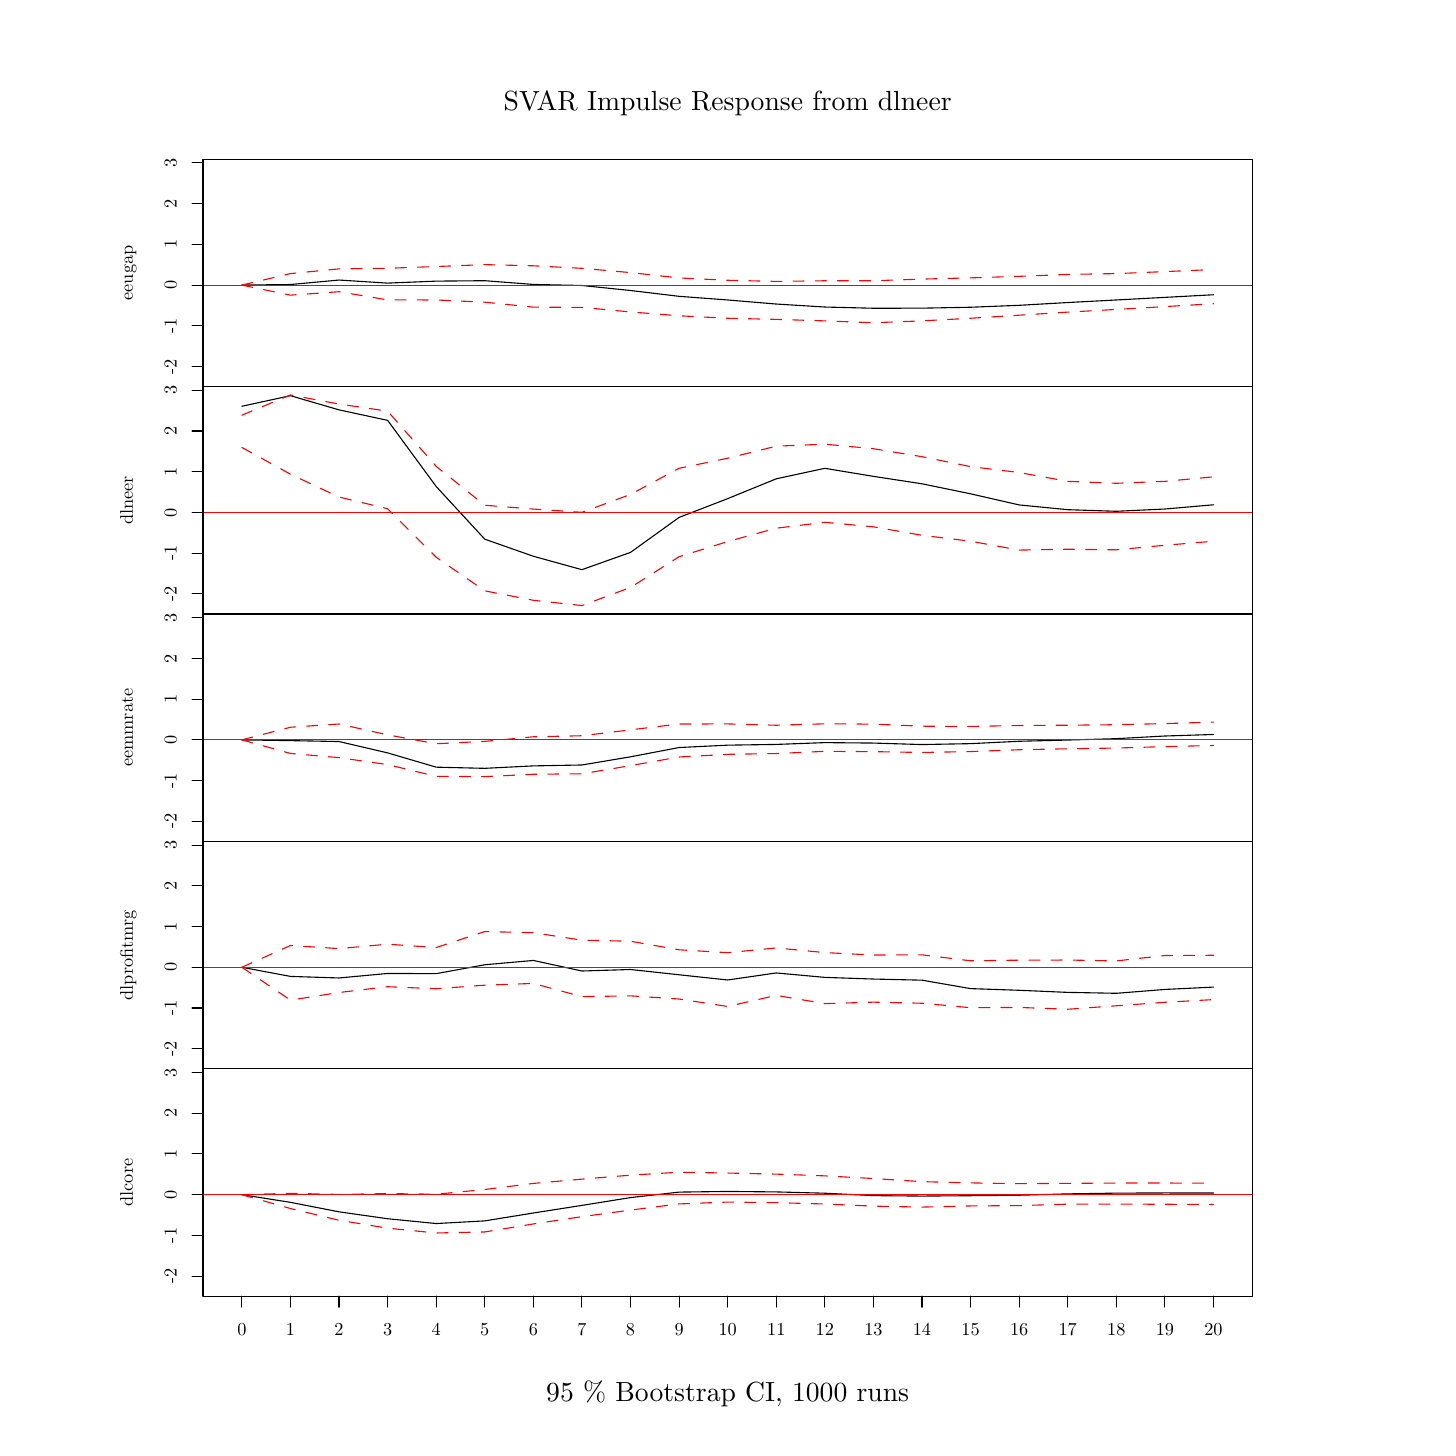
\begin{tikzpicture}[x=1pt,y=1pt]
\definecolor{fillColor}{RGB}{255,255,255}
\path[use as bounding box,fill=fillColor,fill opacity=0.00] (0,0) rectangle (505.89,505.89);
\begin{scope}
\path[clip] ( 63.36,376.20) rectangle (442.53,458.37);
\definecolor{drawColor}{RGB}{0,0,0}

\path[draw=drawColor,line width= 0.4pt,line join=round,line cap=round] ( 77.40,412.87) --
	( 94.96,413.07) --
	(112.51,414.69) --
	(130.07,413.58) --
	(147.62,414.30) --
	(165.17,414.45) --
	(182.73,413.10) --
	(200.28,412.72) --
	(217.84,410.91) --
	(235.39,408.81) --
	(252.94,407.49) --
	(270.50,406.02) --
	(288.05,404.94) --
	(305.61,404.50) --
	(323.16,404.53) --
	(340.72,404.86) --
	(358.27,405.56) --
	(375.82,406.56) --
	(393.38,407.49) --
	(410.93,408.43) --
	(428.49,409.37);
\end{scope}
\begin{scope}
\path[clip] ( 31.68,376.20) rectangle (474.21,458.37);
\definecolor{drawColor}{RGB}{0,0,0}

\node[text=drawColor,anchor=base,inner sep=0pt, outer sep=0pt, scale=  0.66] at (252.94,346.10) {xy{\$}x};

\node[text=drawColor,rotate= 90.00,anchor=base,inner sep=0pt, outer sep=0pt, scale=  0.66] at ( 38.02,417.29) {eeugap};
\end{scope}
\begin{scope}
\path[clip] (  0.00,  0.00) rectangle (505.89,505.89);
\definecolor{drawColor}{RGB}{0,0,0}

\path[draw=drawColor,line width= 0.4pt,line join=round,line cap=round] ( 63.36,383.44) -- ( 63.36,457.02);

\path[draw=drawColor,line width= 0.4pt,line join=round,line cap=round] ( 63.36,383.44) -- ( 59.40,383.44);

\path[draw=drawColor,line width= 0.4pt,line join=round,line cap=round] ( 63.36,398.16) -- ( 59.40,398.16);

\path[draw=drawColor,line width= 0.4pt,line join=round,line cap=round] ( 63.36,412.87) -- ( 59.40,412.87);

\path[draw=drawColor,line width= 0.4pt,line join=round,line cap=round] ( 63.36,427.59) -- ( 59.40,427.59);

\path[draw=drawColor,line width= 0.4pt,line join=round,line cap=round] ( 63.36,442.30) -- ( 59.40,442.30);

\path[draw=drawColor,line width= 0.4pt,line join=round,line cap=round] ( 63.36,457.02) -- ( 59.40,457.02);

\node[text=drawColor,rotate= 90.00,anchor=base,inner sep=0pt, outer sep=0pt, scale=  0.66] at ( 53.86,383.44) {-2};

\node[text=drawColor,rotate= 90.00,anchor=base,inner sep=0pt, outer sep=0pt, scale=  0.66] at ( 53.86,398.16) {-1};

\node[text=drawColor,rotate= 90.00,anchor=base,inner sep=0pt, outer sep=0pt, scale=  0.66] at ( 53.86,412.87) {0};

\node[text=drawColor,rotate= 90.00,anchor=base,inner sep=0pt, outer sep=0pt, scale=  0.66] at ( 53.86,427.59) {1};

\node[text=drawColor,rotate= 90.00,anchor=base,inner sep=0pt, outer sep=0pt, scale=  0.66] at ( 53.86,442.30) {2};

\node[text=drawColor,rotate= 90.00,anchor=base,inner sep=0pt, outer sep=0pt, scale=  0.66] at ( 53.86,457.02) {3};
\end{scope}
\begin{scope}
\path[clip] ( 63.36,376.20) rectangle (442.53,458.37);
\definecolor{drawColor}{RGB}{255,0,0}

\path[draw=drawColor,line width= 0.4pt,line join=round,line cap=round] ( 63.36,412.87) -- (442.53,412.87);

\path[draw=drawColor,line width= 0.4pt,dash pattern=on 4pt off 4pt ,line join=round,line cap=round] ( 77.40,412.87) --
	( 94.96,417.03) --
	(112.51,418.73) --
	(130.07,418.94) --
	(147.62,419.58) --
	(165.17,420.26) --
	(182.73,419.84) --
	(200.28,418.93) --
	(217.84,417.38) --
	(235.39,415.45) --
	(252.94,414.61) --
	(270.50,414.20) --
	(288.05,414.43) --
	(305.61,414.44) --
	(323.16,415.03) --
	(340.72,415.48) --
	(358.27,416.03) --
	(375.82,416.72) --
	(393.38,417.02) --
	(410.93,417.74) --
	(428.49,418.49);

\path[draw=drawColor,line width= 0.4pt,dash pattern=on 4pt off 4pt ,line join=round,line cap=round] ( 77.40,412.87) --
	( 94.96,409.23) --
	(112.51,410.47) --
	(130.07,407.52) --
	(147.62,407.49) --
	(165.17,406.69) --
	(182.73,404.90) --
	(200.28,404.82) --
	(217.84,403.16) --
	(235.39,401.78) --
	(252.94,400.88) --
	(270.50,400.48) --
	(288.05,399.93) --
	(305.61,399.26) --
	(323.16,399.94) --
	(340.72,400.88) --
	(358.27,401.99) --
	(375.82,403.10) --
	(393.38,404.07) --
	(410.93,405.10) --
	(428.49,406.13);
\end{scope}
\begin{scope}
\path[clip] (  0.00,  0.00) rectangle (505.89,505.89);
\definecolor{drawColor}{RGB}{0,0,0}

\path[draw=drawColor,line width= 0.4pt,line join=round,line cap=round] ( 63.36,376.20) --
	(442.53,376.20) --
	(442.53,458.37) --
	( 63.36,458.37) --
	( 63.36,376.20);
\end{scope}
\begin{scope}
\path[clip] ( 63.36,294.03) rectangle (442.53,376.20);
\definecolor{drawColor}{RGB}{0,0,0}

\path[draw=drawColor,line width= 0.4pt,line join=round,line cap=round] ( 77.40,369.08) --
	( 94.96,372.90) --
	(112.51,367.78) --
	(130.07,363.99) --
	(147.62,340.08) --
	(165.17,321.05) --
	(182.73,314.88) --
	(200.28,310.03) --
	(217.84,316.28) --
	(235.39,328.92) --
	(252.94,335.70) --
	(270.50,342.87) --
	(288.05,346.66) --
	(305.61,343.75) --
	(323.16,341.07) --
	(340.72,337.44) --
	(358.27,333.43) --
	(375.82,331.71) --
	(393.38,331.13) --
	(410.93,331.95) --
	(428.49,333.48);
\end{scope}
\begin{scope}
\path[clip] ( 31.68,294.03) rectangle (474.21,376.20);
\definecolor{drawColor}{RGB}{0,0,0}

\node[text=drawColor,anchor=base,inner sep=0pt, outer sep=0pt, scale=  0.66] at (252.94,263.93) {xy{\$}x};

\node[text=drawColor,rotate= 90.00,anchor=base,inner sep=0pt, outer sep=0pt, scale=  0.66] at ( 38.02,335.12) {dlneer};
\end{scope}
\begin{scope}
\path[clip] (  0.00,  0.00) rectangle (505.89,505.89);
\definecolor{drawColor}{RGB}{0,0,0}

\path[draw=drawColor,line width= 0.4pt,line join=round,line cap=round] ( 63.36,301.27) -- ( 63.36,374.85);

\path[draw=drawColor,line width= 0.4pt,line join=round,line cap=round] ( 63.36,301.27) -- ( 59.40,301.27);

\path[draw=drawColor,line width= 0.4pt,line join=round,line cap=round] ( 63.36,315.99) -- ( 59.40,315.99);

\path[draw=drawColor,line width= 0.4pt,line join=round,line cap=round] ( 63.36,330.70) -- ( 59.40,330.70);

\path[draw=drawColor,line width= 0.4pt,line join=round,line cap=round] ( 63.36,345.42) -- ( 59.40,345.42);

\path[draw=drawColor,line width= 0.4pt,line join=round,line cap=round] ( 63.36,360.13) -- ( 59.40,360.13);

\path[draw=drawColor,line width= 0.4pt,line join=round,line cap=round] ( 63.36,374.85) -- ( 59.40,374.85);

\node[text=drawColor,rotate= 90.00,anchor=base,inner sep=0pt, outer sep=0pt, scale=  0.66] at ( 53.86,301.27) {-2};

\node[text=drawColor,rotate= 90.00,anchor=base,inner sep=0pt, outer sep=0pt, scale=  0.66] at ( 53.86,315.99) {-1};

\node[text=drawColor,rotate= 90.00,anchor=base,inner sep=0pt, outer sep=0pt, scale=  0.66] at ( 53.86,330.70) {0};

\node[text=drawColor,rotate= 90.00,anchor=base,inner sep=0pt, outer sep=0pt, scale=  0.66] at ( 53.86,345.42) {1};

\node[text=drawColor,rotate= 90.00,anchor=base,inner sep=0pt, outer sep=0pt, scale=  0.66] at ( 53.86,360.13) {2};

\node[text=drawColor,rotate= 90.00,anchor=base,inner sep=0pt, outer sep=0pt, scale=  0.66] at ( 53.86,374.85) {3};
\end{scope}
\begin{scope}
\path[clip] ( 63.36,294.03) rectangle (442.53,376.20);
\definecolor{drawColor}{RGB}{255,0,0}

\path[draw=drawColor,line width= 0.4pt,line join=round,line cap=round] ( 63.36,330.70) -- (442.53,330.70);

\path[draw=drawColor,line width= 0.4pt,dash pattern=on 4pt off 4pt ,line join=round,line cap=round] ( 77.40,365.85) --
	( 94.96,373.16) --
	(112.51,369.89) --
	(130.07,367.32) --
	(147.62,347.37) --
	(165.17,333.31) --
	(182.73,331.94) --
	(200.28,330.76) --
	(217.84,337.23) --
	(235.39,346.67) --
	(252.94,350.30) --
	(270.50,354.66) --
	(288.05,355.38) --
	(305.61,353.75) --
	(323.16,350.86) --
	(340.72,347.27) --
	(358.27,345.15) --
	(375.82,341.95) --
	(393.38,341.25) --
	(410.93,341.95) --
	(428.49,343.58);

\path[draw=drawColor,line width= 0.4pt,dash pattern=on 4pt off 4pt ,line join=round,line cap=round] ( 77.40,354.21) --
	( 94.96,344.53) --
	(112.51,336.28) --
	(130.07,332.06) --
	(147.62,314.53) --
	(165.17,302.39) --
	(182.73,298.97) --
	(200.28,297.07) --
	(217.84,303.61) --
	(235.39,314.71) --
	(252.94,320.20) --
	(270.50,325.02) --
	(288.05,327.16) --
	(305.61,325.52) --
	(323.16,322.46) --
	(340.72,320.32) --
	(358.27,317.11) --
	(375.82,317.42) --
	(393.38,317.21) --
	(410.93,318.85) --
	(428.49,320.31);
\end{scope}
\begin{scope}
\path[clip] (  0.00,  0.00) rectangle (505.89,505.89);
\definecolor{drawColor}{RGB}{0,0,0}

\path[draw=drawColor,line width= 0.4pt,line join=round,line cap=round] ( 63.36,294.03) --
	(442.53,294.03) --
	(442.53,376.20) --
	( 63.36,376.20) --
	( 63.36,294.03);
\end{scope}
\begin{scope}
\path[clip] ( 63.36,211.86) rectangle (442.53,294.03);
\definecolor{drawColor}{RGB}{0,0,0}

\path[draw=drawColor,line width= 0.4pt,line join=round,line cap=round] ( 77.40,248.53) --
	( 94.96,248.26) --
	(112.51,247.93) --
	(130.07,243.83) --
	(147.62,238.67) --
	(165.17,238.25) --
	(182.73,239.13) --
	(200.28,239.46) --
	(217.84,242.41) --
	(235.39,245.77) --
	(252.94,246.62) --
	(270.50,246.89) --
	(288.05,247.54) --
	(305.61,247.38) --
	(323.16,246.84) --
	(340.72,247.17) --
	(358.27,248.03) --
	(375.82,248.47) --
	(393.38,248.97) --
	(410.93,249.93) --
	(428.49,250.48);
\end{scope}
\begin{scope}
\path[clip] ( 31.68,211.86) rectangle (474.21,294.03);
\definecolor{drawColor}{RGB}{0,0,0}

\node[text=drawColor,anchor=base,inner sep=0pt, outer sep=0pt, scale=  0.66] at (252.94,181.76) {xy{\$}x};

\node[text=drawColor,rotate= 90.00,anchor=base,inner sep=0pt, outer sep=0pt, scale=  0.66] at ( 38.02,252.94) {eemmrate};
\end{scope}
\begin{scope}
\path[clip] (  0.00,  0.00) rectangle (505.89,505.89);
\definecolor{drawColor}{RGB}{0,0,0}

\path[draw=drawColor,line width= 0.4pt,line join=round,line cap=round] ( 63.36,219.10) -- ( 63.36,292.68);

\path[draw=drawColor,line width= 0.4pt,line join=round,line cap=round] ( 63.36,219.10) -- ( 59.40,219.10);

\path[draw=drawColor,line width= 0.4pt,line join=round,line cap=round] ( 63.36,233.82) -- ( 59.40,233.82);

\path[draw=drawColor,line width= 0.4pt,line join=round,line cap=round] ( 63.36,248.53) -- ( 59.40,248.53);

\path[draw=drawColor,line width= 0.4pt,line join=round,line cap=round] ( 63.36,263.25) -- ( 59.40,263.25);

\path[draw=drawColor,line width= 0.4pt,line join=round,line cap=round] ( 63.36,277.96) -- ( 59.40,277.96);

\path[draw=drawColor,line width= 0.4pt,line join=round,line cap=round] ( 63.36,292.68) -- ( 59.40,292.68);

\node[text=drawColor,rotate= 90.00,anchor=base,inner sep=0pt, outer sep=0pt, scale=  0.66] at ( 53.86,219.10) {-2};

\node[text=drawColor,rotate= 90.00,anchor=base,inner sep=0pt, outer sep=0pt, scale=  0.66] at ( 53.86,233.82) {-1};

\node[text=drawColor,rotate= 90.00,anchor=base,inner sep=0pt, outer sep=0pt, scale=  0.66] at ( 53.86,248.53) {0};

\node[text=drawColor,rotate= 90.00,anchor=base,inner sep=0pt, outer sep=0pt, scale=  0.66] at ( 53.86,263.25) {1};

\node[text=drawColor,rotate= 90.00,anchor=base,inner sep=0pt, outer sep=0pt, scale=  0.66] at ( 53.86,277.96) {2};

\node[text=drawColor,rotate= 90.00,anchor=base,inner sep=0pt, outer sep=0pt, scale=  0.66] at ( 53.86,292.68) {3};
\end{scope}
\begin{scope}
\path[clip] ( 63.36,211.86) rectangle (442.53,294.03);
\definecolor{drawColor}{RGB}{255,0,0}

\path[draw=drawColor,line width= 0.4pt,line join=round,line cap=round] ( 63.36,248.53) -- (442.53,248.53);

\path[draw=drawColor,line width= 0.4pt,dash pattern=on 4pt off 4pt ,line join=round,line cap=round] ( 77.40,248.53) --
	( 94.96,253.10) --
	(112.51,254.27) --
	(130.07,250.35) --
	(147.62,247.13) --
	(165.17,248.00) --
	(182.73,249.65) --
	(200.28,250.02) --
	(217.84,252.16) --
	(235.39,254.27) --
	(252.94,254.30) --
	(270.50,253.82) --
	(288.05,254.34) --
	(305.61,254.22) --
	(323.16,253.48) --
	(340.72,253.39) --
	(358.27,253.72) --
	(375.82,253.83) --
	(393.38,254.01) --
	(410.93,254.42) --
	(428.49,254.95);

\path[draw=drawColor,line width= 0.4pt,dash pattern=on 4pt off 4pt ,line join=round,line cap=round] ( 77.40,248.53) --
	( 94.96,243.63) --
	(112.51,242.11) --
	(130.07,239.60) --
	(147.62,235.35) --
	(165.17,235.24) --
	(182.73,236.11) --
	(200.28,236.27) --
	(217.84,239.23) --
	(235.39,242.35) --
	(252.94,243.31) --
	(270.50,243.59) --
	(288.05,244.39) --
	(305.61,244.28) --
	(323.16,243.98) --
	(340.72,244.31) --
	(358.27,244.97) --
	(375.82,245.32) --
	(393.38,245.58) --
	(410.93,246.10) --
	(428.49,246.50);
\end{scope}
\begin{scope}
\path[clip] (  0.00,  0.00) rectangle (505.89,505.89);
\definecolor{drawColor}{RGB}{0,0,0}

\path[draw=drawColor,line width= 0.4pt,line join=round,line cap=round] ( 63.36,211.86) --
	(442.53,211.86) --
	(442.53,294.03) --
	( 63.36,294.03) --
	( 63.36,211.86);
\end{scope}
\begin{scope}
\path[clip] ( 63.36,129.69) rectangle (442.53,211.86);
\definecolor{drawColor}{RGB}{0,0,0}

\path[draw=drawColor,line width= 0.4pt,line join=round,line cap=round] ( 77.40,166.36) --
	( 94.96,163.06) --
	(112.51,162.50) --
	(130.07,164.13) --
	(147.62,164.06) --
	(165.17,167.27) --
	(182.73,168.83) --
	(200.28,165.01) --
	(217.84,165.56) --
	(235.39,163.65) --
	(252.94,161.77) --
	(270.50,164.31) --
	(288.05,162.71) --
	(305.61,162.11) --
	(323.16,161.70) --
	(340.72,158.65) --
	(358.27,158.05) --
	(375.82,157.29) --
	(393.38,156.96) --
	(410.93,158.35) --
	(428.49,159.20);
\end{scope}
\begin{scope}
\path[clip] ( 31.68,129.69) rectangle (474.21,211.86);
\definecolor{drawColor}{RGB}{0,0,0}

\node[text=drawColor,anchor=base,inner sep=0pt, outer sep=0pt, scale=  0.66] at (252.94, 99.59) {xy{\$}x};

\node[text=drawColor,rotate= 90.00,anchor=base,inner sep=0pt, outer sep=0pt, scale=  0.66] at ( 38.02,170.77) {dlprofitmrg};
\end{scope}
\begin{scope}
\path[clip] (  0.00,  0.00) rectangle (505.89,505.89);
\definecolor{drawColor}{RGB}{0,0,0}

\path[draw=drawColor,line width= 0.4pt,line join=round,line cap=round] ( 63.36,136.93) -- ( 63.36,210.51);

\path[draw=drawColor,line width= 0.4pt,line join=round,line cap=round] ( 63.36,136.93) -- ( 59.40,136.93);

\path[draw=drawColor,line width= 0.4pt,line join=round,line cap=round] ( 63.36,151.65) -- ( 59.40,151.65);

\path[draw=drawColor,line width= 0.4pt,line join=round,line cap=round] ( 63.36,166.36) -- ( 59.40,166.36);

\path[draw=drawColor,line width= 0.4pt,line join=round,line cap=round] ( 63.36,181.08) -- ( 59.40,181.08);

\path[draw=drawColor,line width= 0.4pt,line join=round,line cap=round] ( 63.36,195.79) -- ( 59.40,195.79);

\path[draw=drawColor,line width= 0.4pt,line join=round,line cap=round] ( 63.36,210.51) -- ( 59.40,210.51);

\node[text=drawColor,rotate= 90.00,anchor=base,inner sep=0pt, outer sep=0pt, scale=  0.66] at ( 53.86,136.93) {-2};

\node[text=drawColor,rotate= 90.00,anchor=base,inner sep=0pt, outer sep=0pt, scale=  0.66] at ( 53.86,151.65) {-1};

\node[text=drawColor,rotate= 90.00,anchor=base,inner sep=0pt, outer sep=0pt, scale=  0.66] at ( 53.86,166.36) {0};

\node[text=drawColor,rotate= 90.00,anchor=base,inner sep=0pt, outer sep=0pt, scale=  0.66] at ( 53.86,181.08) {1};

\node[text=drawColor,rotate= 90.00,anchor=base,inner sep=0pt, outer sep=0pt, scale=  0.66] at ( 53.86,195.79) {2};

\node[text=drawColor,rotate= 90.00,anchor=base,inner sep=0pt, outer sep=0pt, scale=  0.66] at ( 53.86,210.51) {3};
\end{scope}
\begin{scope}
\path[clip] ( 63.36,129.69) rectangle (442.53,211.86);
\definecolor{drawColor}{RGB}{255,0,0}

\path[draw=drawColor,line width= 0.4pt,line join=round,line cap=round] ( 63.36,166.36) -- (442.53,166.36);

\path[draw=drawColor,line width= 0.4pt,dash pattern=on 4pt off 4pt ,line join=round,line cap=round] ( 77.40,166.36) --
	( 94.96,174.24) --
	(112.51,173.11) --
	(130.07,174.71) --
	(147.62,173.49) --
	(165.17,179.26) --
	(182.73,178.86) --
	(200.28,176.16) --
	(217.84,175.77) --
	(235.39,172.68) --
	(252.94,171.64) --
	(270.50,173.35) --
	(288.05,171.67) --
	(305.61,170.78) --
	(323.16,170.86) --
	(340.72,168.70) --
	(358.27,168.93) --
	(375.82,168.98) --
	(393.38,168.66) --
	(410.93,170.60) --
	(428.49,170.70);

\path[draw=drawColor,line width= 0.4pt,dash pattern=on 4pt off 4pt ,line join=round,line cap=round] ( 77.40,166.36) --
	( 94.96,154.50) --
	(112.51,157.24) --
	(130.07,159.34) --
	(147.62,158.60) --
	(165.17,159.90) --
	(182.73,160.52) --
	(200.28,155.75) --
	(217.84,156.04) --
	(235.39,154.89) --
	(252.94,152.20) --
	(270.50,156.21) --
	(288.05,153.23) --
	(305.61,153.76) --
	(323.16,153.37) --
	(340.72,151.75) --
	(358.27,151.85) --
	(375.82,151.20) --
	(393.38,152.45) --
	(410.93,153.72) --
	(428.49,154.68);
\end{scope}
\begin{scope}
\path[clip] (  0.00,  0.00) rectangle (505.89,505.89);
\definecolor{drawColor}{RGB}{0,0,0}

\path[draw=drawColor,line width= 0.4pt,line join=round,line cap=round] ( 63.36,129.69) --
	(442.53,129.69) --
	(442.53,211.86) --
	( 63.36,211.86) --
	( 63.36,129.69);
\end{scope}
\begin{scope}
\path[clip] ( 63.36, 47.52) rectangle (442.53,129.69);
\definecolor{drawColor}{RGB}{0,0,0}

\path[draw=drawColor,line width= 0.4pt,line join=round,line cap=round] ( 77.40, 84.19) --
	( 94.96, 81.42) --
	(112.51, 77.99) --
	(130.07, 75.50) --
	(147.62, 73.76) --
	(165.17, 74.72) --
	(182.73, 77.57) --
	(200.28, 80.32) --
	(217.84, 83.14) --
	(235.39, 85.12) --
	(252.94, 85.36) --
	(270.50, 85.19) --
	(288.05, 84.72) --
	(305.61, 83.85) --
	(323.16, 83.68) --
	(340.72, 83.82) --
	(358.27, 83.99) --
	(375.82, 84.48) --
	(393.38, 84.75) --
	(410.93, 84.82) --
	(428.49, 84.79);
\end{scope}
\begin{scope}
\path[clip] ( 31.68, 47.52) rectangle (474.21,129.69);
\definecolor{drawColor}{RGB}{0,0,0}

\node[text=drawColor,anchor=base,inner sep=0pt, outer sep=0pt, scale=  0.66] at (252.94, 17.42) {xy{\$}x};

\node[text=drawColor,rotate= 90.00,anchor=base,inner sep=0pt, outer sep=0pt, scale=  0.66] at ( 38.02, 88.60) {dlcore};
\end{scope}
\begin{scope}
\path[clip] (  0.00,  0.00) rectangle (505.89,505.89);
\definecolor{drawColor}{RGB}{0,0,0}

\path[draw=drawColor,line width= 0.4pt,line join=round,line cap=round] ( 63.36, 54.76) -- ( 63.36,128.34);

\path[draw=drawColor,line width= 0.4pt,line join=round,line cap=round] ( 63.36, 54.76) -- ( 59.40, 54.76);

\path[draw=drawColor,line width= 0.4pt,line join=round,line cap=round] ( 63.36, 69.48) -- ( 59.40, 69.48);

\path[draw=drawColor,line width= 0.4pt,line join=round,line cap=round] ( 63.36, 84.19) -- ( 59.40, 84.19);

\path[draw=drawColor,line width= 0.4pt,line join=round,line cap=round] ( 63.36, 98.91) -- ( 59.40, 98.91);

\path[draw=drawColor,line width= 0.4pt,line join=round,line cap=round] ( 63.36,113.62) -- ( 59.40,113.62);

\path[draw=drawColor,line width= 0.4pt,line join=round,line cap=round] ( 63.36,128.34) -- ( 59.40,128.34);

\node[text=drawColor,rotate= 90.00,anchor=base,inner sep=0pt, outer sep=0pt, scale=  0.66] at ( 53.86, 54.76) {-2};

\node[text=drawColor,rotate= 90.00,anchor=base,inner sep=0pt, outer sep=0pt, scale=  0.66] at ( 53.86, 69.48) {-1};

\node[text=drawColor,rotate= 90.00,anchor=base,inner sep=0pt, outer sep=0pt, scale=  0.66] at ( 53.86, 84.19) {0};

\node[text=drawColor,rotate= 90.00,anchor=base,inner sep=0pt, outer sep=0pt, scale=  0.66] at ( 53.86, 98.91) {1};

\node[text=drawColor,rotate= 90.00,anchor=base,inner sep=0pt, outer sep=0pt, scale=  0.66] at ( 53.86,113.62) {2};

\node[text=drawColor,rotate= 90.00,anchor=base,inner sep=0pt, outer sep=0pt, scale=  0.66] at ( 53.86,128.34) {3};

\path[draw=drawColor,line width= 0.4pt,line join=round,line cap=round] ( 77.40, 47.52) -- (428.49, 47.52);

\path[draw=drawColor,line width= 0.4pt,line join=round,line cap=round] ( 77.40, 47.52) -- ( 77.40, 43.56);

\path[draw=drawColor,line width= 0.4pt,line join=round,line cap=round] ( 94.96, 47.52) -- ( 94.96, 43.56);

\path[draw=drawColor,line width= 0.4pt,line join=round,line cap=round] (112.51, 47.52) -- (112.51, 43.56);

\path[draw=drawColor,line width= 0.4pt,line join=round,line cap=round] (130.07, 47.52) -- (130.07, 43.56);

\path[draw=drawColor,line width= 0.4pt,line join=round,line cap=round] (147.62, 47.52) -- (147.62, 43.56);

\path[draw=drawColor,line width= 0.4pt,line join=round,line cap=round] (165.17, 47.52) -- (165.17, 43.56);

\path[draw=drawColor,line width= 0.4pt,line join=round,line cap=round] (182.73, 47.52) -- (182.73, 43.56);

\path[draw=drawColor,line width= 0.4pt,line join=round,line cap=round] (200.28, 47.52) -- (200.28, 43.56);

\path[draw=drawColor,line width= 0.4pt,line join=round,line cap=round] (217.84, 47.52) -- (217.84, 43.56);

\path[draw=drawColor,line width= 0.4pt,line join=round,line cap=round] (235.39, 47.52) -- (235.39, 43.56);

\path[draw=drawColor,line width= 0.4pt,line join=round,line cap=round] (252.94, 47.52) -- (252.94, 43.56);

\path[draw=drawColor,line width= 0.4pt,line join=round,line cap=round] (270.50, 47.52) -- (270.50, 43.56);

\path[draw=drawColor,line width= 0.4pt,line join=round,line cap=round] (288.05, 47.52) -- (288.05, 43.56);

\path[draw=drawColor,line width= 0.4pt,line join=round,line cap=round] (305.61, 47.52) -- (305.61, 43.56);

\path[draw=drawColor,line width= 0.4pt,line join=round,line cap=round] (323.16, 47.52) -- (323.16, 43.56);

\path[draw=drawColor,line width= 0.4pt,line join=round,line cap=round] (340.72, 47.52) -- (340.72, 43.56);

\path[draw=drawColor,line width= 0.4pt,line join=round,line cap=round] (358.27, 47.52) -- (358.27, 43.56);

\path[draw=drawColor,line width= 0.4pt,line join=round,line cap=round] (375.82, 47.52) -- (375.82, 43.56);

\path[draw=drawColor,line width= 0.4pt,line join=round,line cap=round] (393.38, 47.52) -- (393.38, 43.56);

\path[draw=drawColor,line width= 0.4pt,line join=round,line cap=round] (410.93, 47.52) -- (410.93, 43.56);

\path[draw=drawColor,line width= 0.4pt,line join=round,line cap=round] (428.49, 47.52) -- (428.49, 43.56);

\node[text=drawColor,anchor=base,inner sep=0pt, outer sep=0pt, scale=  0.66] at ( 77.40, 33.26) {0};

\node[text=drawColor,anchor=base,inner sep=0pt, outer sep=0pt, scale=  0.66] at ( 94.96, 33.26) {1};

\node[text=drawColor,anchor=base,inner sep=0pt, outer sep=0pt, scale=  0.66] at (112.51, 33.26) {2};

\node[text=drawColor,anchor=base,inner sep=0pt, outer sep=0pt, scale=  0.66] at (130.07, 33.26) {3};

\node[text=drawColor,anchor=base,inner sep=0pt, outer sep=0pt, scale=  0.66] at (147.62, 33.26) {4};

\node[text=drawColor,anchor=base,inner sep=0pt, outer sep=0pt, scale=  0.66] at (165.17, 33.26) {5};

\node[text=drawColor,anchor=base,inner sep=0pt, outer sep=0pt, scale=  0.66] at (182.73, 33.26) {6};

\node[text=drawColor,anchor=base,inner sep=0pt, outer sep=0pt, scale=  0.66] at (200.28, 33.26) {7};

\node[text=drawColor,anchor=base,inner sep=0pt, outer sep=0pt, scale=  0.66] at (217.84, 33.26) {8};

\node[text=drawColor,anchor=base,inner sep=0pt, outer sep=0pt, scale=  0.66] at (235.39, 33.26) {9};

\node[text=drawColor,anchor=base,inner sep=0pt, outer sep=0pt, scale=  0.66] at (252.94, 33.26) {10};

\node[text=drawColor,anchor=base,inner sep=0pt, outer sep=0pt, scale=  0.66] at (270.50, 33.26) {11};

\node[text=drawColor,anchor=base,inner sep=0pt, outer sep=0pt, scale=  0.66] at (288.05, 33.26) {12};

\node[text=drawColor,anchor=base,inner sep=0pt, outer sep=0pt, scale=  0.66] at (305.61, 33.26) {13};

\node[text=drawColor,anchor=base,inner sep=0pt, outer sep=0pt, scale=  0.66] at (323.16, 33.26) {14};

\node[text=drawColor,anchor=base,inner sep=0pt, outer sep=0pt, scale=  0.66] at (340.72, 33.26) {15};

\node[text=drawColor,anchor=base,inner sep=0pt, outer sep=0pt, scale=  0.66] at (358.27, 33.26) {16};

\node[text=drawColor,anchor=base,inner sep=0pt, outer sep=0pt, scale=  0.66] at (375.82, 33.26) {17};

\node[text=drawColor,anchor=base,inner sep=0pt, outer sep=0pt, scale=  0.66] at (393.38, 33.26) {18};

\node[text=drawColor,anchor=base,inner sep=0pt, outer sep=0pt, scale=  0.66] at (410.93, 33.26) {19};

\node[text=drawColor,anchor=base,inner sep=0pt, outer sep=0pt, scale=  0.66] at (428.49, 33.26) {20};

\path[draw=drawColor,line width= 0.4pt,line join=round,line cap=round] ( 63.36, 47.52) --
	(442.53, 47.52) --
	(442.53,129.69) --
	( 63.36,129.69) --
	( 63.36, 47.52);
\end{scope}
\begin{scope}
\path[clip] ( 63.36, 47.52) rectangle (442.53,129.69);
\definecolor{drawColor}{RGB}{255,0,0}

\path[draw=drawColor,line width= 0.4pt,line join=round,line cap=round] ( 63.36, 84.19) -- (442.53, 84.19);

\path[draw=drawColor,line width= 0.4pt,dash pattern=on 4pt off 4pt ,line join=round,line cap=round] ( 77.40, 84.19) --
	( 94.96, 84.68) --
	(112.51, 84.28) --
	(130.07, 84.58) --
	(147.62, 84.36) --
	(165.17, 86.06) --
	(182.73, 88.26) --
	(200.28, 89.81) --
	(217.84, 91.24) --
	(235.39, 92.31) --
	(252.94, 92.01) --
	(270.50, 91.62) --
	(288.05, 90.99) --
	(305.61, 90.03) --
	(323.16, 88.90) --
	(340.72, 88.45) --
	(358.27, 88.16) --
	(375.82, 88.29) --
	(393.38, 88.39) --
	(410.93, 88.40) --
	(428.49, 88.35);

\path[draw=drawColor,line width= 0.4pt,dash pattern=on 4pt off 4pt ,line join=round,line cap=round] ( 77.40, 84.19) --
	( 94.96, 79.19) --
	(112.51, 74.95) --
	(130.07, 72.09) --
	(147.62, 70.35) --
	(165.17, 70.72) --
	(182.73, 73.62) --
	(200.28, 76.25) --
	(217.84, 78.63) --
	(235.39, 80.85) --
	(252.94, 81.52) --
	(270.50, 81.31) --
	(288.05, 80.82) --
	(305.61, 80.05) --
	(323.16, 79.70) --
	(340.72, 80.12) --
	(358.27, 80.24) --
	(375.82, 80.76) --
	(393.38, 80.81) --
	(410.93, 80.72) --
	(428.49, 80.68);
\end{scope}
\begin{scope}
\path[clip] (  0.00,  0.00) rectangle (505.89,505.89);
\definecolor{drawColor}{RGB}{0,0,0}

\node[text=drawColor,anchor=base,inner sep=0pt, outer sep=0pt, scale=  1.00] at (252.94,475.79) {SVAR Impulse Response from dlneer};

\node[text=drawColor,anchor=base,inner sep=0pt, outer sep=0pt, scale=  1.00] at (252.94,  9.50) {95 {\%} Bootstrap CI,  1000 runs};
\end{scope}
\end{tikzpicture}
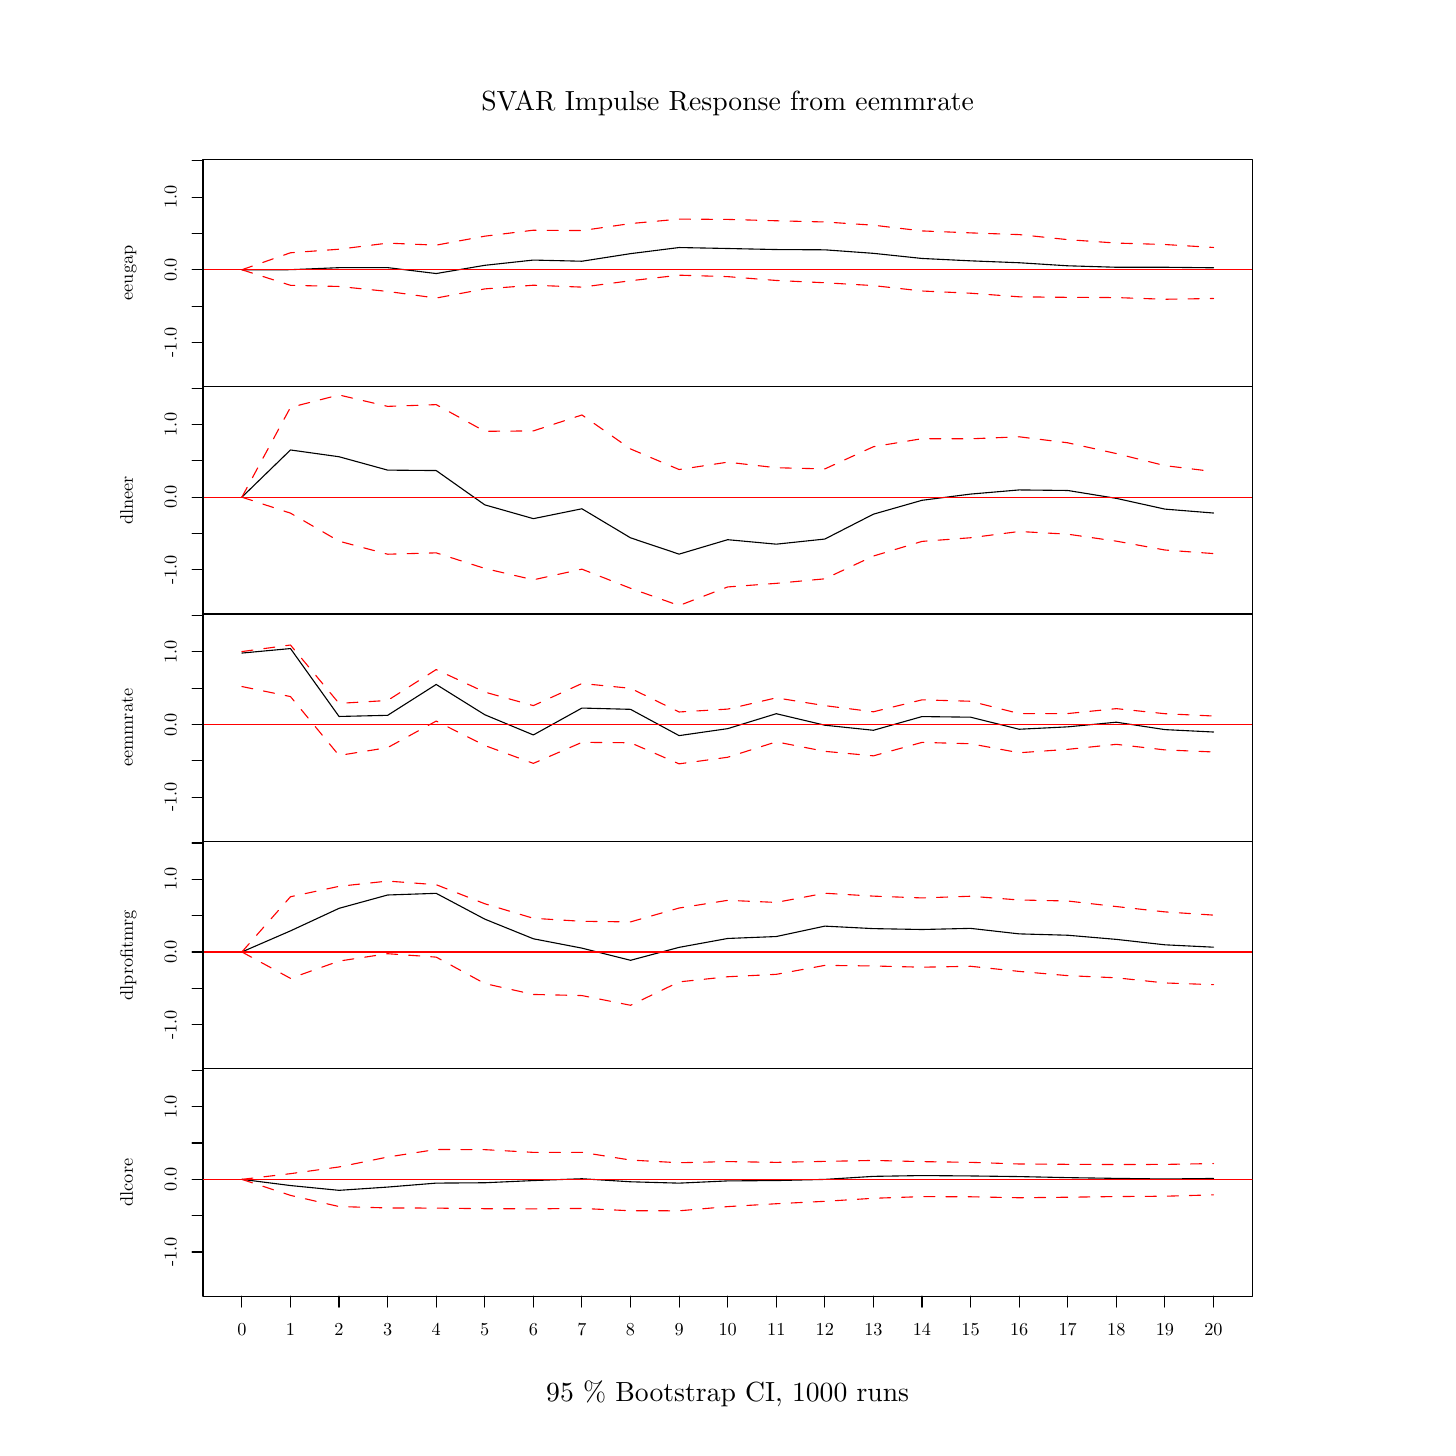
\begin{tikzpicture}[x=1pt,y=1pt]
\definecolor{fillColor}{RGB}{255,255,255}
\path[use as bounding box,fill=fillColor,fill opacity=0.00] (0,0) rectangle (505.89,505.89);
\begin{scope}
\path[clip] ( 63.36,376.20) rectangle (442.53,458.37);
\definecolor{drawColor}{RGB}{0,0,0}

\path[draw=drawColor,line width= 0.4pt,line join=round,line cap=round] ( 77.40,418.41) --
	( 94.96,418.43) --
	(112.51,419.16) --
	(130.07,419.18) --
	(147.62,417.04) --
	(165.17,420.01) --
	(182.73,421.91) --
	(200.28,421.49) --
	(217.84,424.23) --
	(235.39,426.44) --
	(252.94,426.09) --
	(270.50,425.71) --
	(288.05,425.61) --
	(305.61,424.34) --
	(323.16,422.49) --
	(340.72,421.63) --
	(358.27,420.94) --
	(375.82,419.84) --
	(393.38,419.31) --
	(410.93,419.31) --
	(428.49,419.12);
\end{scope}
\begin{scope}
\path[clip] ( 31.68,376.20) rectangle (474.21,458.37);
\definecolor{drawColor}{RGB}{0,0,0}

\node[text=drawColor,anchor=base,inner sep=0pt, outer sep=0pt, scale=  0.66] at (252.94,346.10) {xy{\$}x};

\node[text=drawColor,rotate= 90.00,anchor=base,inner sep=0pt, outer sep=0pt, scale=  0.66] at ( 38.02,417.29) {eeugap};
\end{scope}
\begin{scope}
\path[clip] (  0.00,  0.00) rectangle (505.89,505.89);
\definecolor{drawColor}{RGB}{0,0,0}

\path[draw=drawColor,line width= 0.4pt,line join=round,line cap=round] ( 63.36,392.16) -- ( 63.36,457.79);

\path[draw=drawColor,line width= 0.4pt,line join=round,line cap=round] ( 63.36,392.16) -- ( 59.40,392.16);

\path[draw=drawColor,line width= 0.4pt,line join=round,line cap=round] ( 63.36,405.29) -- ( 59.40,405.29);

\path[draw=drawColor,line width= 0.4pt,line join=round,line cap=round] ( 63.36,418.41) -- ( 59.40,418.41);

\path[draw=drawColor,line width= 0.4pt,line join=round,line cap=round] ( 63.36,431.54) -- ( 59.40,431.54);

\path[draw=drawColor,line width= 0.4pt,line join=round,line cap=round] ( 63.36,444.66) -- ( 59.40,444.66);

\path[draw=drawColor,line width= 0.4pt,line join=round,line cap=round] ( 63.36,457.79) -- ( 59.40,457.79);

\node[text=drawColor,rotate= 90.00,anchor=base,inner sep=0pt, outer sep=0pt, scale=  0.66] at ( 53.86,392.16) {-1.0};

\node[text=drawColor,rotate= 90.00,anchor=base,inner sep=0pt, outer sep=0pt, scale=  0.66] at ( 53.86,418.41) {0.0};

\node[text=drawColor,rotate= 90.00,anchor=base,inner sep=0pt, outer sep=0pt, scale=  0.66] at ( 53.86,444.66) {1.0};
\end{scope}
\begin{scope}
\path[clip] ( 63.36,376.20) rectangle (442.53,458.37);
\definecolor{drawColor}{RGB}{255,0,0}

\path[draw=drawColor,line width= 0.4pt,line join=round,line cap=round] ( 63.36,418.41) -- (442.53,418.41);

\path[draw=drawColor,line width= 0.4pt,dash pattern=on 4pt off 4pt ,line join=round,line cap=round] ( 77.40,418.41) --
	( 94.96,424.54) --
	(112.51,425.83) --
	(130.07,428.03) --
	(147.62,427.30) --
	(165.17,430.54) --
	(182.73,432.70) --
	(200.28,432.57) --
	(217.84,435.10) --
	(235.39,436.70) --
	(252.94,436.60) --
	(270.50,436.11) --
	(288.05,435.67) --
	(305.61,434.51) --
	(323.16,432.44) --
	(340.72,431.73) --
	(358.27,431.11) --
	(375.82,429.29) --
	(393.38,428.05) --
	(410.93,427.53) --
	(428.49,426.46);

\path[draw=drawColor,line width= 0.4pt,dash pattern=on 4pt off 4pt ,line join=round,line cap=round] ( 77.40,418.41) --
	( 94.96,412.79) --
	(112.51,412.37) --
	(130.07,410.58) --
	(147.62,408.18) --
	(165.17,411.49) --
	(182.73,412.82) --
	(200.28,412.13) --
	(217.84,414.44) --
	(235.39,416.45) --
	(252.94,415.92) --
	(270.50,414.54) --
	(288.05,413.71) --
	(305.61,412.69) --
	(323.16,410.73) --
	(340.72,409.93) --
	(358.27,408.63) --
	(375.82,408.44) --
	(393.38,408.35) --
	(410.93,407.75) --
	(428.49,408.02);
\end{scope}
\begin{scope}
\path[clip] (  0.00,  0.00) rectangle (505.89,505.89);
\definecolor{drawColor}{RGB}{0,0,0}

\path[draw=drawColor,line width= 0.4pt,line join=round,line cap=round] ( 63.36,376.20) --
	(442.53,376.20) --
	(442.53,458.37) --
	( 63.36,458.37) --
	( 63.36,376.20);
\end{scope}
\begin{scope}
\path[clip] ( 63.36,294.03) rectangle (442.53,376.20);
\definecolor{drawColor}{RGB}{0,0,0}

\path[draw=drawColor,line width= 0.4pt,line join=round,line cap=round] ( 77.40,336.24) --
	( 94.96,353.29) --
	(112.51,350.84) --
	(130.07,346.01) --
	(147.62,345.85) --
	(165.17,333.46) --
	(182.73,328.47) --
	(200.28,332.04) --
	(217.84,321.54) --
	(235.39,315.65) --
	(252.94,320.87) --
	(270.50,319.25) --
	(288.05,321.10) --
	(305.61,330.09) --
	(323.16,335.10) --
	(340.72,337.35) --
	(358.27,338.85) --
	(375.82,338.65) --
	(393.38,335.80) --
	(410.93,331.92) --
	(428.49,330.50);
\end{scope}
\begin{scope}
\path[clip] ( 31.68,294.03) rectangle (474.21,376.20);
\definecolor{drawColor}{RGB}{0,0,0}

\node[text=drawColor,anchor=base,inner sep=0pt, outer sep=0pt, scale=  0.66] at (252.94,263.93) {xy{\$}x};

\node[text=drawColor,rotate= 90.00,anchor=base,inner sep=0pt, outer sep=0pt, scale=  0.66] at ( 38.02,335.12) {dlneer};
\end{scope}
\begin{scope}
\path[clip] (  0.00,  0.00) rectangle (505.89,505.89);
\definecolor{drawColor}{RGB}{0,0,0}

\path[draw=drawColor,line width= 0.4pt,line join=round,line cap=round] ( 63.36,309.99) -- ( 63.36,375.62);

\path[draw=drawColor,line width= 0.4pt,line join=round,line cap=round] ( 63.36,309.99) -- ( 59.40,309.99);

\path[draw=drawColor,line width= 0.4pt,line join=round,line cap=round] ( 63.36,323.12) -- ( 59.40,323.12);

\path[draw=drawColor,line width= 0.4pt,line join=round,line cap=round] ( 63.36,336.24) -- ( 59.40,336.24);

\path[draw=drawColor,line width= 0.4pt,line join=round,line cap=round] ( 63.36,349.37) -- ( 59.40,349.37);

\path[draw=drawColor,line width= 0.4pt,line join=round,line cap=round] ( 63.36,362.49) -- ( 59.40,362.49);

\path[draw=drawColor,line width= 0.4pt,line join=round,line cap=round] ( 63.36,375.62) -- ( 59.40,375.62);

\node[text=drawColor,rotate= 90.00,anchor=base,inner sep=0pt, outer sep=0pt, scale=  0.66] at ( 53.86,309.99) {-1.0};

\node[text=drawColor,rotate= 90.00,anchor=base,inner sep=0pt, outer sep=0pt, scale=  0.66] at ( 53.86,336.24) {0.0};

\node[text=drawColor,rotate= 90.00,anchor=base,inner sep=0pt, outer sep=0pt, scale=  0.66] at ( 53.86,362.49) {1.0};
\end{scope}
\begin{scope}
\path[clip] ( 63.36,294.03) rectangle (442.53,376.20);
\definecolor{drawColor}{RGB}{255,0,0}

\path[draw=drawColor,line width= 0.4pt,line join=round,line cap=round] ( 63.36,336.24) -- (442.53,336.24);

\path[draw=drawColor,line width= 0.4pt,dash pattern=on 4pt off 4pt ,line join=round,line cap=round] ( 77.40,336.24) --
	( 94.96,368.68) --
	(112.51,373.16) --
	(130.07,369.04) --
	(147.62,369.67) --
	(165.17,360.04) --
	(182.73,360.17) --
	(200.28,365.94) --
	(217.84,353.66) --
	(235.39,346.22) --
	(252.94,348.88) --
	(270.50,346.87) --
	(288.05,346.44) --
	(305.61,354.46) --
	(323.16,357.37) --
	(340.72,357.32) --
	(358.27,358.05) --
	(375.82,355.88) --
	(393.38,351.99) --
	(410.93,347.63) --
	(428.49,345.48);

\path[draw=drawColor,line width= 0.4pt,dash pattern=on 4pt off 4pt ,line join=round,line cap=round] ( 77.40,336.24) --
	( 94.96,330.46) --
	(112.51,320.33) --
	(130.07,315.62) --
	(147.62,316.11) --
	(165.17,310.48) --
	(182.73,306.37) --
	(200.28,310.22) --
	(217.84,303.31) --
	(235.39,297.07) --
	(252.94,303.79) --
	(270.50,305.09) --
	(288.05,306.73) --
	(305.61,314.96) --
	(323.16,320.25) --
	(340.72,321.57) --
	(358.27,323.83) --
	(375.82,322.86) --
	(393.38,320.34) --
	(410.93,317.14) --
	(428.49,315.85);
\end{scope}
\begin{scope}
\path[clip] (  0.00,  0.00) rectangle (505.89,505.89);
\definecolor{drawColor}{RGB}{0,0,0}

\path[draw=drawColor,line width= 0.4pt,line join=round,line cap=round] ( 63.36,294.03) --
	(442.53,294.03) --
	(442.53,376.20) --
	( 63.36,376.20) --
	( 63.36,294.03);
\end{scope}
\begin{scope}
\path[clip] ( 63.36,211.86) rectangle (442.53,294.03);
\definecolor{drawColor}{RGB}{0,0,0}

\path[draw=drawColor,line width= 0.4pt,line join=round,line cap=round] ( 77.40,279.90) --
	( 94.96,281.53) --
	(112.51,256.99) --
	(130.07,257.40) --
	(147.62,268.56) --
	(165.17,257.62) --
	(182.73,250.31) --
	(200.28,260.03) --
	(217.84,259.57) --
	(235.39,250.07) --
	(252.94,252.59) --
	(270.50,257.99) --
	(288.05,253.83) --
	(305.61,252.00) --
	(323.16,256.95) --
	(340.72,256.73) --
	(358.27,252.37) --
	(375.82,253.24) --
	(393.38,254.92) --
	(410.93,252.24) --
	(428.49,251.37);
\end{scope}
\begin{scope}
\path[clip] ( 31.68,211.86) rectangle (474.21,294.03);
\definecolor{drawColor}{RGB}{0,0,0}

\node[text=drawColor,anchor=base,inner sep=0pt, outer sep=0pt, scale=  0.66] at (252.94,181.76) {xy{\$}x};

\node[text=drawColor,rotate= 90.00,anchor=base,inner sep=0pt, outer sep=0pt, scale=  0.66] at ( 38.02,252.94) {eemmrate};
\end{scope}
\begin{scope}
\path[clip] (  0.00,  0.00) rectangle (505.89,505.89);
\definecolor{drawColor}{RGB}{0,0,0}

\path[draw=drawColor,line width= 0.4pt,line join=round,line cap=round] ( 63.36,227.82) -- ( 63.36,293.45);

\path[draw=drawColor,line width= 0.4pt,line join=round,line cap=round] ( 63.36,227.82) -- ( 59.40,227.82);

\path[draw=drawColor,line width= 0.4pt,line join=round,line cap=round] ( 63.36,240.95) -- ( 59.40,240.95);

\path[draw=drawColor,line width= 0.4pt,line join=round,line cap=round] ( 63.36,254.07) -- ( 59.40,254.07);

\path[draw=drawColor,line width= 0.4pt,line join=round,line cap=round] ( 63.36,267.20) -- ( 59.40,267.20);

\path[draw=drawColor,line width= 0.4pt,line join=round,line cap=round] ( 63.36,280.32) -- ( 59.40,280.32);

\path[draw=drawColor,line width= 0.4pt,line join=round,line cap=round] ( 63.36,293.45) -- ( 59.40,293.45);

\node[text=drawColor,rotate= 90.00,anchor=base,inner sep=0pt, outer sep=0pt, scale=  0.66] at ( 53.86,227.82) {-1.0};

\node[text=drawColor,rotate= 90.00,anchor=base,inner sep=0pt, outer sep=0pt, scale=  0.66] at ( 53.86,254.07) {0.0};

\node[text=drawColor,rotate= 90.00,anchor=base,inner sep=0pt, outer sep=0pt, scale=  0.66] at ( 53.86,280.32) {1.0};
\end{scope}
\begin{scope}
\path[clip] ( 63.36,211.86) rectangle (442.53,294.03);
\definecolor{drawColor}{RGB}{255,0,0}

\path[draw=drawColor,line width= 0.4pt,line join=round,line cap=round] ( 63.36,254.07) -- (442.53,254.07);

\path[draw=drawColor,line width= 0.4pt,dash pattern=on 4pt off 4pt ,line join=round,line cap=round] ( 77.40,280.44) --
	( 94.96,282.81) --
	(112.51,261.72) --
	(130.07,262.77) --
	(147.62,273.95) --
	(165.17,265.80) --
	(182.73,260.91) --
	(200.28,268.90) --
	(217.84,267.17) --
	(235.39,258.61) --
	(252.94,259.65) --
	(270.50,263.72) --
	(288.05,260.90) --
	(305.61,258.68) --
	(323.16,263.00) --
	(340.72,262.49) --
	(358.27,258.04) --
	(375.82,258.04) --
	(393.38,259.82) --
	(410.93,257.99) --
	(428.49,257.15);

\path[draw=drawColor,line width= 0.4pt,dash pattern=on 4pt off 4pt ,line join=round,line cap=round] ( 77.40,267.81) --
	( 94.96,264.18) --
	(112.51,242.90) --
	(130.07,245.73) --
	(147.62,255.33) --
	(165.17,246.50) --
	(182.73,240.04) --
	(200.28,247.64) --
	(217.84,247.49) --
	(235.39,239.87) --
	(252.94,242.25) --
	(270.50,247.82) --
	(288.05,244.39) --
	(305.61,242.76) --
	(323.16,247.62) --
	(340.72,247.14) --
	(358.27,243.88) --
	(375.82,245.11) --
	(393.38,246.92) --
	(410.93,244.91) --
	(428.49,244.16);
\end{scope}
\begin{scope}
\path[clip] (  0.00,  0.00) rectangle (505.89,505.89);
\definecolor{drawColor}{RGB}{0,0,0}

\path[draw=drawColor,line width= 0.4pt,line join=round,line cap=round] ( 63.36,211.86) --
	(442.53,211.86) --
	(442.53,294.03) --
	( 63.36,294.03) --
	( 63.36,211.86);
\end{scope}
\begin{scope}
\path[clip] ( 63.36,129.69) rectangle (442.53,211.86);
\definecolor{drawColor}{RGB}{0,0,0}

\path[draw=drawColor,line width= 0.4pt,line join=round,line cap=round] ( 77.40,171.90) --
	( 94.96,179.51) --
	(112.51,187.66) --
	(130.07,192.48) --
	(147.62,193.08) --
	(165.17,183.76) --
	(182.73,176.66) --
	(200.28,173.28) --
	(217.84,168.88) --
	(235.39,173.56) --
	(252.94,176.77) --
	(270.50,177.47) --
	(288.05,181.23) --
	(305.61,180.33) --
	(323.16,180.01) --
	(340.72,180.42) --
	(358.27,178.43) --
	(375.82,177.94) --
	(393.38,176.44) --
	(410.93,174.48) --
	(428.49,173.62);
\end{scope}
\begin{scope}
\path[clip] ( 31.68,129.69) rectangle (474.21,211.86);
\definecolor{drawColor}{RGB}{0,0,0}

\node[text=drawColor,anchor=base,inner sep=0pt, outer sep=0pt, scale=  0.66] at (252.94, 99.59) {xy{\$}x};

\node[text=drawColor,rotate= 90.00,anchor=base,inner sep=0pt, outer sep=0pt, scale=  0.66] at ( 38.02,170.77) {dlprofitmrg};
\end{scope}
\begin{scope}
\path[clip] (  0.00,  0.00) rectangle (505.89,505.89);
\definecolor{drawColor}{RGB}{0,0,0}

\path[draw=drawColor,line width= 0.4pt,line join=round,line cap=round] ( 63.36,145.65) -- ( 63.36,211.28);

\path[draw=drawColor,line width= 0.4pt,line join=round,line cap=round] ( 63.36,145.65) -- ( 59.40,145.65);

\path[draw=drawColor,line width= 0.4pt,line join=round,line cap=round] ( 63.36,158.78) -- ( 59.40,158.78);

\path[draw=drawColor,line width= 0.4pt,line join=round,line cap=round] ( 63.36,171.90) -- ( 59.40,171.90);

\path[draw=drawColor,line width= 0.4pt,line join=round,line cap=round] ( 63.36,185.03) -- ( 59.40,185.03);

\path[draw=drawColor,line width= 0.4pt,line join=round,line cap=round] ( 63.36,198.15) -- ( 59.40,198.15);

\path[draw=drawColor,line width= 0.4pt,line join=round,line cap=round] ( 63.36,211.28) -- ( 59.40,211.28);

\node[text=drawColor,rotate= 90.00,anchor=base,inner sep=0pt, outer sep=0pt, scale=  0.66] at ( 53.86,145.65) {-1.0};

\node[text=drawColor,rotate= 90.00,anchor=base,inner sep=0pt, outer sep=0pt, scale=  0.66] at ( 53.86,171.90) {0.0};

\node[text=drawColor,rotate= 90.00,anchor=base,inner sep=0pt, outer sep=0pt, scale=  0.66] at ( 53.86,198.15) {1.0};
\end{scope}
\begin{scope}
\path[clip] ( 63.36,129.69) rectangle (442.53,211.86);
\definecolor{drawColor}{RGB}{255,0,0}

\path[draw=drawColor,line width= 0.4pt,line join=round,line cap=round] ( 63.36,171.90) -- (442.53,171.90);

\path[draw=drawColor,line width= 0.4pt,dash pattern=on 4pt off 4pt ,line join=round,line cap=round] ( 77.40,171.90) --
	( 94.96,191.84) --
	(112.51,195.61) --
	(130.07,197.51) --
	(147.62,196.20) --
	(165.17,189.32) --
	(182.73,184.06) --
	(200.28,182.97) --
	(217.84,182.76) --
	(235.39,187.77) --
	(252.94,190.55) --
	(270.50,189.80) --
	(288.05,193.12) --
	(305.61,192.07) --
	(323.16,191.42) --
	(340.72,192.03) --
	(358.27,190.68) --
	(375.82,190.31) --
	(393.38,188.30) --
	(410.93,186.38) --
	(428.49,185.21);

\path[draw=drawColor,line width= 0.4pt,dash pattern=on 4pt off 4pt ,line join=round,line cap=round] ( 77.40,171.90) --
	( 94.96,162.36) --
	(112.51,168.60) --
	(130.07,171.27) --
	(147.62,170.03) --
	(165.17,160.48) --
	(182.73,156.54) --
	(200.28,156.14) --
	(217.84,152.63) --
	(235.39,161.08) --
	(252.94,162.94) --
	(270.50,163.81) --
	(288.05,167.05) --
	(305.61,166.83) --
	(323.16,166.39) --
	(340.72,166.72) --
	(358.27,164.87) --
	(375.82,163.34) --
	(393.38,162.56) --
	(410.93,160.70) --
	(428.49,160.07);
\end{scope}
\begin{scope}
\path[clip] (  0.00,  0.00) rectangle (505.89,505.89);
\definecolor{drawColor}{RGB}{0,0,0}

\path[draw=drawColor,line width= 0.4pt,line join=round,line cap=round] ( 63.36,129.69) --
	(442.53,129.69) --
	(442.53,211.86) --
	( 63.36,211.86) --
	( 63.36,129.69);
\end{scope}
\begin{scope}
\path[clip] ( 63.36, 47.52) rectangle (442.53,129.69);
\definecolor{drawColor}{RGB}{0,0,0}

\path[draw=drawColor,line width= 0.4pt,line join=round,line cap=round] ( 77.40, 89.73) --
	( 94.96, 87.49) --
	(112.51, 85.76) --
	(130.07, 86.94) --
	(147.62, 88.37) --
	(165.17, 88.50) --
	(182.73, 89.29) --
	(200.28, 89.95) --
	(217.84, 88.85) --
	(235.39, 88.36) --
	(252.94, 89.17) --
	(270.50, 89.29) --
	(288.05, 89.71) --
	(305.61, 90.81) --
	(323.16, 91.10) --
	(340.72, 90.96) --
	(358.27, 90.73) --
	(375.82, 90.35) --
	(393.38, 90.08) --
	(410.93, 89.86) --
	(428.49, 90.05);
\end{scope}
\begin{scope}
\path[clip] ( 31.68, 47.52) rectangle (474.21,129.69);
\definecolor{drawColor}{RGB}{0,0,0}

\node[text=drawColor,anchor=base,inner sep=0pt, outer sep=0pt, scale=  0.66] at (252.94, 17.42) {xy{\$}x};

\node[text=drawColor,rotate= 90.00,anchor=base,inner sep=0pt, outer sep=0pt, scale=  0.66] at ( 38.02, 88.60) {dlcore};
\end{scope}
\begin{scope}
\path[clip] (  0.00,  0.00) rectangle (505.89,505.89);
\definecolor{drawColor}{RGB}{0,0,0}

\path[draw=drawColor,line width= 0.4pt,line join=round,line cap=round] ( 63.36, 63.48) -- ( 63.36,129.11);

\path[draw=drawColor,line width= 0.4pt,line join=round,line cap=round] ( 63.36, 63.48) -- ( 59.40, 63.48);

\path[draw=drawColor,line width= 0.4pt,line join=round,line cap=round] ( 63.36, 76.61) -- ( 59.40, 76.61);

\path[draw=drawColor,line width= 0.4pt,line join=round,line cap=round] ( 63.36, 89.73) -- ( 59.40, 89.73);

\path[draw=drawColor,line width= 0.4pt,line join=round,line cap=round] ( 63.36,102.86) -- ( 59.40,102.86);

\path[draw=drawColor,line width= 0.4pt,line join=round,line cap=round] ( 63.36,115.98) -- ( 59.40,115.98);

\path[draw=drawColor,line width= 0.4pt,line join=round,line cap=round] ( 63.36,129.11) -- ( 59.40,129.11);

\node[text=drawColor,rotate= 90.00,anchor=base,inner sep=0pt, outer sep=0pt, scale=  0.66] at ( 53.86, 63.48) {-1.0};

\node[text=drawColor,rotate= 90.00,anchor=base,inner sep=0pt, outer sep=0pt, scale=  0.66] at ( 53.86, 89.73) {0.0};

\node[text=drawColor,rotate= 90.00,anchor=base,inner sep=0pt, outer sep=0pt, scale=  0.66] at ( 53.86,115.98) {1.0};

\path[draw=drawColor,line width= 0.4pt,line join=round,line cap=round] ( 77.40, 47.52) -- (428.49, 47.52);

\path[draw=drawColor,line width= 0.4pt,line join=round,line cap=round] ( 77.40, 47.52) -- ( 77.40, 43.56);

\path[draw=drawColor,line width= 0.4pt,line join=round,line cap=round] ( 94.96, 47.52) -- ( 94.96, 43.56);

\path[draw=drawColor,line width= 0.4pt,line join=round,line cap=round] (112.51, 47.52) -- (112.51, 43.56);

\path[draw=drawColor,line width= 0.4pt,line join=round,line cap=round] (130.07, 47.52) -- (130.07, 43.56);

\path[draw=drawColor,line width= 0.4pt,line join=round,line cap=round] (147.62, 47.52) -- (147.62, 43.56);

\path[draw=drawColor,line width= 0.4pt,line join=round,line cap=round] (165.17, 47.52) -- (165.17, 43.56);

\path[draw=drawColor,line width= 0.4pt,line join=round,line cap=round] (182.73, 47.52) -- (182.73, 43.56);

\path[draw=drawColor,line width= 0.4pt,line join=round,line cap=round] (200.28, 47.52) -- (200.28, 43.56);

\path[draw=drawColor,line width= 0.4pt,line join=round,line cap=round] (217.84, 47.52) -- (217.84, 43.56);

\path[draw=drawColor,line width= 0.4pt,line join=round,line cap=round] (235.39, 47.52) -- (235.39, 43.56);

\path[draw=drawColor,line width= 0.4pt,line join=round,line cap=round] (252.94, 47.52) -- (252.94, 43.56);

\path[draw=drawColor,line width= 0.4pt,line join=round,line cap=round] (270.50, 47.52) -- (270.50, 43.56);

\path[draw=drawColor,line width= 0.4pt,line join=round,line cap=round] (288.05, 47.52) -- (288.05, 43.56);

\path[draw=drawColor,line width= 0.4pt,line join=round,line cap=round] (305.61, 47.52) -- (305.61, 43.56);

\path[draw=drawColor,line width= 0.4pt,line join=round,line cap=round] (323.16, 47.52) -- (323.16, 43.56);

\path[draw=drawColor,line width= 0.4pt,line join=round,line cap=round] (340.72, 47.52) -- (340.72, 43.56);

\path[draw=drawColor,line width= 0.4pt,line join=round,line cap=round] (358.27, 47.52) -- (358.27, 43.56);

\path[draw=drawColor,line width= 0.4pt,line join=round,line cap=round] (375.82, 47.52) -- (375.82, 43.56);

\path[draw=drawColor,line width= 0.4pt,line join=round,line cap=round] (393.38, 47.52) -- (393.38, 43.56);

\path[draw=drawColor,line width= 0.4pt,line join=round,line cap=round] (410.93, 47.52) -- (410.93, 43.56);

\path[draw=drawColor,line width= 0.4pt,line join=round,line cap=round] (428.49, 47.52) -- (428.49, 43.56);

\node[text=drawColor,anchor=base,inner sep=0pt, outer sep=0pt, scale=  0.66] at ( 77.40, 33.26) {0};

\node[text=drawColor,anchor=base,inner sep=0pt, outer sep=0pt, scale=  0.66] at ( 94.96, 33.26) {1};

\node[text=drawColor,anchor=base,inner sep=0pt, outer sep=0pt, scale=  0.66] at (112.51, 33.26) {2};

\node[text=drawColor,anchor=base,inner sep=0pt, outer sep=0pt, scale=  0.66] at (130.07, 33.26) {3};

\node[text=drawColor,anchor=base,inner sep=0pt, outer sep=0pt, scale=  0.66] at (147.62, 33.26) {4};

\node[text=drawColor,anchor=base,inner sep=0pt, outer sep=0pt, scale=  0.66] at (165.17, 33.26) {5};

\node[text=drawColor,anchor=base,inner sep=0pt, outer sep=0pt, scale=  0.66] at (182.73, 33.26) {6};

\node[text=drawColor,anchor=base,inner sep=0pt, outer sep=0pt, scale=  0.66] at (200.28, 33.26) {7};

\node[text=drawColor,anchor=base,inner sep=0pt, outer sep=0pt, scale=  0.66] at (217.84, 33.26) {8};

\node[text=drawColor,anchor=base,inner sep=0pt, outer sep=0pt, scale=  0.66] at (235.39, 33.26) {9};

\node[text=drawColor,anchor=base,inner sep=0pt, outer sep=0pt, scale=  0.66] at (252.94, 33.26) {10};

\node[text=drawColor,anchor=base,inner sep=0pt, outer sep=0pt, scale=  0.66] at (270.50, 33.26) {11};

\node[text=drawColor,anchor=base,inner sep=0pt, outer sep=0pt, scale=  0.66] at (288.05, 33.26) {12};

\node[text=drawColor,anchor=base,inner sep=0pt, outer sep=0pt, scale=  0.66] at (305.61, 33.26) {13};

\node[text=drawColor,anchor=base,inner sep=0pt, outer sep=0pt, scale=  0.66] at (323.16, 33.26) {14};

\node[text=drawColor,anchor=base,inner sep=0pt, outer sep=0pt, scale=  0.66] at (340.72, 33.26) {15};

\node[text=drawColor,anchor=base,inner sep=0pt, outer sep=0pt, scale=  0.66] at (358.27, 33.26) {16};

\node[text=drawColor,anchor=base,inner sep=0pt, outer sep=0pt, scale=  0.66] at (375.82, 33.26) {17};

\node[text=drawColor,anchor=base,inner sep=0pt, outer sep=0pt, scale=  0.66] at (393.38, 33.26) {18};

\node[text=drawColor,anchor=base,inner sep=0pt, outer sep=0pt, scale=  0.66] at (410.93, 33.26) {19};

\node[text=drawColor,anchor=base,inner sep=0pt, outer sep=0pt, scale=  0.66] at (428.49, 33.26) {20};

\path[draw=drawColor,line width= 0.4pt,line join=round,line cap=round] ( 63.36, 47.52) --
	(442.53, 47.52) --
	(442.53,129.69) --
	( 63.36,129.69) --
	( 63.36, 47.52);
\end{scope}
\begin{scope}
\path[clip] ( 63.36, 47.52) rectangle (442.53,129.69);
\definecolor{drawColor}{RGB}{255,0,0}

\path[draw=drawColor,line width= 0.4pt,line join=round,line cap=round] ( 63.36, 89.73) -- (442.53, 89.73);

\path[draw=drawColor,line width= 0.4pt,dash pattern=on 4pt off 4pt ,line join=round,line cap=round] ( 77.40, 89.73) --
	( 94.96, 91.78) --
	(112.51, 94.21) --
	(130.07, 97.79) --
	(147.62,100.53) --
	(165.17,100.46) --
	(182.73, 99.48) --
	(200.28, 99.50) --
	(217.84, 96.70) --
	(235.39, 95.73) --
	(252.94, 96.15) --
	(270.50, 95.87) --
	(288.05, 96.22) --
	(305.61, 96.57) --
	(323.16, 96.13) --
	(340.72, 95.88) --
	(358.27, 95.28) --
	(375.82, 95.16) --
	(393.38, 95.08) --
	(410.93, 95.13) --
	(428.49, 95.44);

\path[draw=drawColor,line width= 0.4pt,dash pattern=on 4pt off 4pt ,line join=round,line cap=round] ( 77.40, 89.73) --
	( 94.96, 83.94) --
	(112.51, 79.90) --
	(130.07, 79.40) --
	(147.62, 79.34) --
	(165.17, 79.12) --
	(182.73, 79.07) --
	(200.28, 79.22) --
	(217.84, 78.38) --
	(235.39, 78.36) --
	(252.94, 79.88) --
	(270.50, 80.92) --
	(288.05, 81.79) --
	(305.61, 82.89) --
	(323.16, 83.49) --
	(340.72, 83.43) --
	(358.27, 83.08) --
	(375.82, 83.27) --
	(393.38, 83.52) --
	(410.93, 83.63) --
	(428.49, 84.13);
\end{scope}
\begin{scope}
\path[clip] (  0.00,  0.00) rectangle (505.89,505.89);
\definecolor{drawColor}{RGB}{0,0,0}

\node[text=drawColor,anchor=base,inner sep=0pt, outer sep=0pt, scale=  1.00] at (252.94,475.79) {SVAR Impulse Response from eemmrate};

\node[text=drawColor,anchor=base,inner sep=0pt, outer sep=0pt, scale=  1.00] at (252.94,  9.50) {95 {\%} Bootstrap CI,  1000 runs};
\end{scope}
\end{tikzpicture}
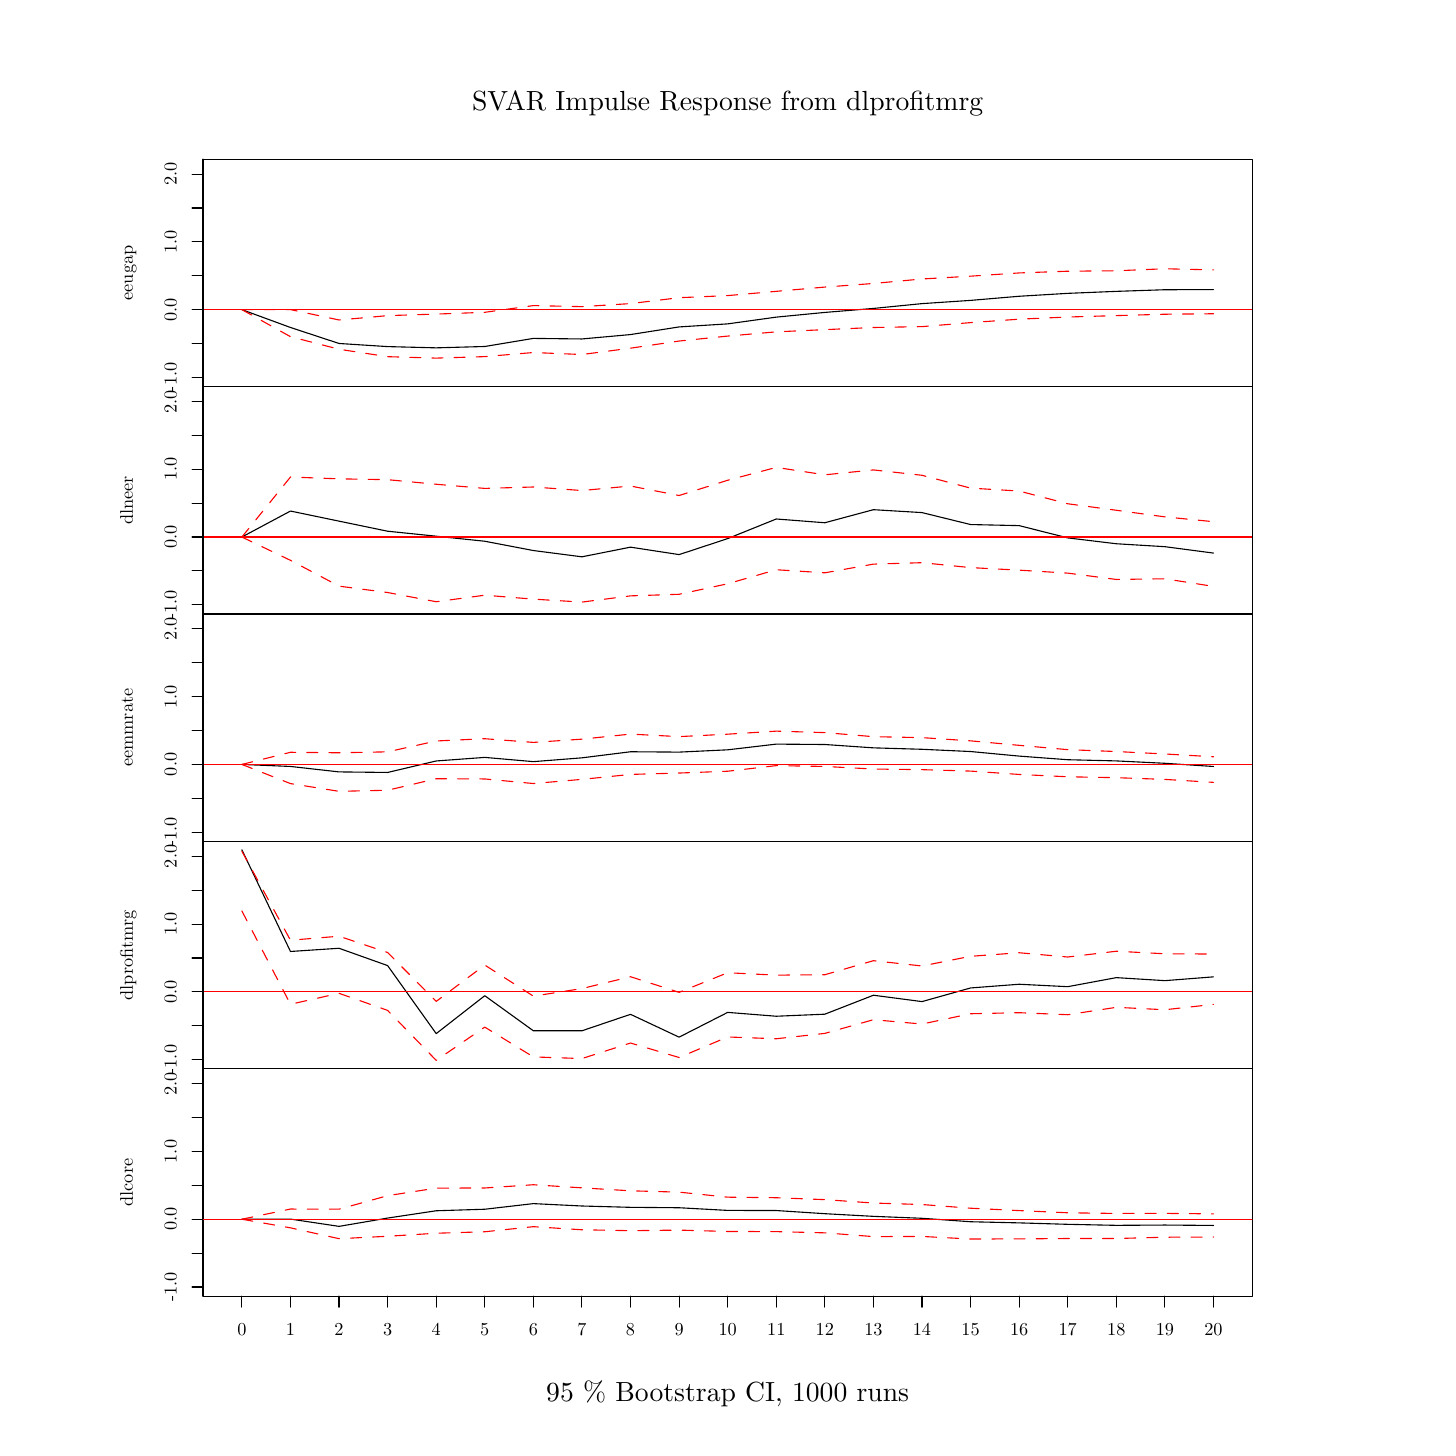
\begin{tikzpicture}[x=1pt,y=1pt]
\definecolor{fillColor}{RGB}{255,255,255}
\path[use as bounding box,fill=fillColor,fill opacity=0.00] (0,0) rectangle (505.89,505.89);
\begin{scope}
\path[clip] ( 63.36,376.20) rectangle (442.53,458.37);
\definecolor{drawColor}{RGB}{0,0,0}

\path[draw=drawColor,line width= 0.4pt,line join=round,line cap=round] ( 77.40,404.00) --
	( 94.96,397.55) --
	(112.51,391.77) --
	(130.07,390.64) --
	(147.62,390.19) --
	(165.17,390.68) --
	(182.73,393.60) --
	(200.28,393.40) --
	(217.84,394.99) --
	(235.39,397.75) --
	(252.94,398.85) --
	(270.50,401.29) --
	(288.05,402.99) --
	(305.61,404.43) --
	(323.16,406.17) --
	(340.72,407.34) --
	(358.27,408.83) --
	(375.82,409.88) --
	(393.38,410.60) --
	(410.93,411.19) --
	(428.49,411.24);
\end{scope}
\begin{scope}
\path[clip] ( 31.68,376.20) rectangle (474.21,458.37);
\definecolor{drawColor}{RGB}{0,0,0}

\node[text=drawColor,anchor=base,inner sep=0pt, outer sep=0pt, scale=  0.66] at (252.94,346.10) {xy{\$}x};

\node[text=drawColor,rotate= 90.00,anchor=base,inner sep=0pt, outer sep=0pt, scale=  0.66] at ( 38.02,417.29) {eeugap};
\end{scope}
\begin{scope}
\path[clip] (  0.00,  0.00) rectangle (505.89,505.89);
\definecolor{drawColor}{RGB}{0,0,0}

\path[draw=drawColor,line width= 0.4pt,line join=round,line cap=round] ( 63.36,379.53) -- ( 63.36,458.37);

\path[draw=drawColor,line width= 0.4pt,line join=round,line cap=round] ( 63.36,379.53) -- ( 59.40,379.53);

\path[draw=drawColor,line width= 0.4pt,line join=round,line cap=round] ( 63.36,391.76) -- ( 59.40,391.76);

\path[draw=drawColor,line width= 0.4pt,line join=round,line cap=round] ( 63.36,404.00) -- ( 59.40,404.00);

\path[draw=drawColor,line width= 0.4pt,line join=round,line cap=round] ( 63.36,416.24) -- ( 59.40,416.24);

\path[draw=drawColor,line width= 0.4pt,line join=round,line cap=round] ( 63.36,428.48) -- ( 59.40,428.48);

\path[draw=drawColor,line width= 0.4pt,line join=round,line cap=round] ( 63.36,440.72) -- ( 59.40,440.72);

\path[draw=drawColor,line width= 0.4pt,line join=round,line cap=round] ( 63.36,452.96) -- ( 59.40,452.96);

\node[text=drawColor,rotate= 90.00,anchor=base,inner sep=0pt, outer sep=0pt, scale=  0.66] at ( 53.86,379.53) {-1.0};

\node[text=drawColor,rotate= 90.00,anchor=base,inner sep=0pt, outer sep=0pt, scale=  0.66] at ( 53.86,404.00) {0.0};

\node[text=drawColor,rotate= 90.00,anchor=base,inner sep=0pt, outer sep=0pt, scale=  0.66] at ( 53.86,428.48) {1.0};

\node[text=drawColor,rotate= 90.00,anchor=base,inner sep=0pt, outer sep=0pt, scale=  0.66] at ( 53.86,452.96) {2.0};
\end{scope}
\begin{scope}
\path[clip] ( 63.36,376.20) rectangle (442.53,458.37);
\definecolor{drawColor}{RGB}{255,0,0}

\path[draw=drawColor,line width= 0.4pt,line join=round,line cap=round] ( 63.36,404.00) -- (442.53,404.00);

\path[draw=drawColor,line width= 0.4pt,dash pattern=on 4pt off 4pt ,line join=round,line cap=round] ( 77.40,404.00) --
	( 94.96,404.02) --
	(112.51,400.26) --
	(130.07,401.83) --
	(147.62,402.39) --
	(165.17,403.03) --
	(182.73,405.46) --
	(200.28,405.08) --
	(217.84,406.18) --
	(235.39,408.31) --
	(252.94,409.07) --
	(270.50,410.61) --
	(288.05,412.15) --
	(305.61,413.45) --
	(323.16,415.07) --
	(340.72,416.09) --
	(358.27,417.26) --
	(375.82,417.88) --
	(393.38,418.04) --
	(410.93,418.77) --
	(428.49,418.35);

\path[draw=drawColor,line width= 0.4pt,dash pattern=on 4pt off 4pt ,line join=round,line cap=round] ( 77.40,404.00) --
	( 94.96,394.23) --
	(112.51,389.68) --
	(130.07,387.00) --
	(147.62,386.48) --
	(165.17,387.02) --
	(182.73,388.50) --
	(200.28,387.78) --
	(217.84,390.07) --
	(235.39,392.65) --
	(252.94,394.44) --
	(270.50,395.97) --
	(288.05,396.77) --
	(305.61,397.54) --
	(323.16,397.86) --
	(340.72,399.31) --
	(358.27,400.55) --
	(375.82,401.33) --
	(393.38,401.84) --
	(410.93,402.34) --
	(428.49,402.51);
\end{scope}
\begin{scope}
\path[clip] (  0.00,  0.00) rectangle (505.89,505.89);
\definecolor{drawColor}{RGB}{0,0,0}

\path[draw=drawColor,line width= 0.4pt,line join=round,line cap=round] ( 63.36,376.20) --
	(442.53,376.20) --
	(442.53,458.37) --
	( 63.36,458.37) --
	( 63.36,376.20);
\end{scope}
\begin{scope}
\path[clip] ( 63.36,294.03) rectangle (442.53,376.20);
\definecolor{drawColor}{RGB}{0,0,0}

\path[draw=drawColor,line width= 0.4pt,line join=round,line cap=round] ( 77.40,321.83) --
	( 94.96,331.22) --
	(112.51,327.57) --
	(130.07,323.93) --
	(147.62,322.13) --
	(165.17,320.31) --
	(182.73,316.95) --
	(200.28,314.68) --
	(217.84,318.17) --
	(235.39,315.48) --
	(252.94,321.26) --
	(270.50,328.35) --
	(288.05,326.99) --
	(305.61,331.71) --
	(323.16,330.66) --
	(340.72,326.34) --
	(358.27,325.95) --
	(375.82,321.52) --
	(393.38,319.40) --
	(410.93,318.34) --
	(428.49,316.03);
\end{scope}
\begin{scope}
\path[clip] ( 31.68,294.03) rectangle (474.21,376.20);
\definecolor{drawColor}{RGB}{0,0,0}

\node[text=drawColor,anchor=base,inner sep=0pt, outer sep=0pt, scale=  0.66] at (252.94,263.93) {xy{\$}x};

\node[text=drawColor,rotate= 90.00,anchor=base,inner sep=0pt, outer sep=0pt, scale=  0.66] at ( 38.02,335.12) {dlneer};
\end{scope}
\begin{scope}
\path[clip] (  0.00,  0.00) rectangle (505.89,505.89);
\definecolor{drawColor}{RGB}{0,0,0}

\path[draw=drawColor,line width= 0.4pt,line join=round,line cap=round] ( 63.36,297.36) -- ( 63.36,376.20);

\path[draw=drawColor,line width= 0.4pt,line join=round,line cap=round] ( 63.36,297.36) -- ( 59.40,297.36);

\path[draw=drawColor,line width= 0.4pt,line join=round,line cap=round] ( 63.36,309.59) -- ( 59.40,309.59);

\path[draw=drawColor,line width= 0.4pt,line join=round,line cap=round] ( 63.36,321.83) -- ( 59.40,321.83);

\path[draw=drawColor,line width= 0.4pt,line join=round,line cap=round] ( 63.36,334.07) -- ( 59.40,334.07);

\path[draw=drawColor,line width= 0.4pt,line join=round,line cap=round] ( 63.36,346.31) -- ( 59.40,346.31);

\path[draw=drawColor,line width= 0.4pt,line join=round,line cap=round] ( 63.36,358.55) -- ( 59.40,358.55);

\path[draw=drawColor,line width= 0.4pt,line join=round,line cap=round] ( 63.36,370.79) -- ( 59.40,370.79);

\node[text=drawColor,rotate= 90.00,anchor=base,inner sep=0pt, outer sep=0pt, scale=  0.66] at ( 53.86,297.36) {-1.0};

\node[text=drawColor,rotate= 90.00,anchor=base,inner sep=0pt, outer sep=0pt, scale=  0.66] at ( 53.86,321.83) {0.0};

\node[text=drawColor,rotate= 90.00,anchor=base,inner sep=0pt, outer sep=0pt, scale=  0.66] at ( 53.86,346.31) {1.0};

\node[text=drawColor,rotate= 90.00,anchor=base,inner sep=0pt, outer sep=0pt, scale=  0.66] at ( 53.86,370.79) {2.0};
\end{scope}
\begin{scope}
\path[clip] ( 63.36,294.03) rectangle (442.53,376.20);
\definecolor{drawColor}{RGB}{255,0,0}

\path[draw=drawColor,line width= 0.4pt,line join=round,line cap=round] ( 63.36,321.83) -- (442.53,321.83);

\path[draw=drawColor,line width= 0.4pt,dash pattern=on 4pt off 4pt ,line join=round,line cap=round] ( 77.40,321.83) --
	( 94.96,343.51) --
	(112.51,342.86) --
	(130.07,342.55) --
	(147.62,340.90) --
	(165.17,339.40) --
	(182.73,339.91) --
	(200.28,338.63) --
	(217.84,340.26) --
	(235.39,336.83) --
	(252.94,342.34) --
	(270.50,346.99) --
	(288.05,344.31) --
	(305.61,346.08) --
	(323.16,344.14) --
	(340.72,339.50) --
	(358.27,338.45) --
	(375.82,333.85) --
	(393.38,331.50) --
	(410.93,329.11) --
	(428.49,327.37);

\path[draw=drawColor,line width= 0.4pt,dash pattern=on 4pt off 4pt ,line join=round,line cap=round] ( 77.40,321.83) --
	( 94.96,313.41) --
	(112.51,304.08) --
	(130.07,301.78) --
	(147.62,298.45) --
	(165.17,300.81) --
	(182.73,299.39) --
	(200.28,298.32) --
	(217.84,300.57) --
	(235.39,301.14) --
	(252.94,304.94) --
	(270.50,310.01) --
	(288.05,308.90) --
	(305.61,312.04) --
	(323.16,312.56) --
	(340.72,310.78) --
	(358.27,309.86) --
	(375.82,308.79) --
	(393.38,306.50) --
	(410.93,306.74) --
	(428.49,303.99);
\end{scope}
\begin{scope}
\path[clip] (  0.00,  0.00) rectangle (505.89,505.89);
\definecolor{drawColor}{RGB}{0,0,0}

\path[draw=drawColor,line width= 0.4pt,line join=round,line cap=round] ( 63.36,294.03) --
	(442.53,294.03) --
	(442.53,376.20) --
	( 63.36,376.20) --
	( 63.36,294.03);
\end{scope}
\begin{scope}
\path[clip] ( 63.36,211.86) rectangle (442.53,294.03);
\definecolor{drawColor}{RGB}{0,0,0}

\path[draw=drawColor,line width= 0.4pt,line join=round,line cap=round] ( 77.40,239.66) --
	( 94.96,238.93) --
	(112.51,236.96) --
	(130.07,236.76) --
	(147.62,240.91) --
	(165.17,242.20) --
	(182.73,240.67) --
	(200.28,242.04) --
	(217.84,244.24) --
	(235.39,244.11) --
	(252.94,244.94) --
	(270.50,247.00) --
	(288.05,246.86) --
	(305.61,245.65) --
	(323.16,245.13) --
	(340.72,244.32) --
	(358.27,242.67) --
	(375.82,241.36) --
	(393.38,240.93) --
	(410.93,240.07) --
	(428.49,238.92);
\end{scope}
\begin{scope}
\path[clip] ( 31.68,211.86) rectangle (474.21,294.03);
\definecolor{drawColor}{RGB}{0,0,0}

\node[text=drawColor,anchor=base,inner sep=0pt, outer sep=0pt, scale=  0.66] at (252.94,181.76) {xy{\$}x};

\node[text=drawColor,rotate= 90.00,anchor=base,inner sep=0pt, outer sep=0pt, scale=  0.66] at ( 38.02,252.94) {eemmrate};
\end{scope}
\begin{scope}
\path[clip] (  0.00,  0.00) rectangle (505.89,505.89);
\definecolor{drawColor}{RGB}{0,0,0}

\path[draw=drawColor,line width= 0.4pt,line join=round,line cap=round] ( 63.36,215.19) -- ( 63.36,294.03);

\path[draw=drawColor,line width= 0.4pt,line join=round,line cap=round] ( 63.36,215.19) -- ( 59.40,215.19);

\path[draw=drawColor,line width= 0.4pt,line join=round,line cap=round] ( 63.36,227.42) -- ( 59.40,227.42);

\path[draw=drawColor,line width= 0.4pt,line join=round,line cap=round] ( 63.36,239.66) -- ( 59.40,239.66);

\path[draw=drawColor,line width= 0.4pt,line join=round,line cap=round] ( 63.36,251.90) -- ( 59.40,251.90);

\path[draw=drawColor,line width= 0.4pt,line join=round,line cap=round] ( 63.36,264.14) -- ( 59.40,264.14);

\path[draw=drawColor,line width= 0.4pt,line join=round,line cap=round] ( 63.36,276.38) -- ( 59.40,276.38);

\path[draw=drawColor,line width= 0.4pt,line join=round,line cap=round] ( 63.36,288.62) -- ( 59.40,288.62);

\node[text=drawColor,rotate= 90.00,anchor=base,inner sep=0pt, outer sep=0pt, scale=  0.66] at ( 53.86,215.19) {-1.0};

\node[text=drawColor,rotate= 90.00,anchor=base,inner sep=0pt, outer sep=0pt, scale=  0.66] at ( 53.86,239.66) {0.0};

\node[text=drawColor,rotate= 90.00,anchor=base,inner sep=0pt, outer sep=0pt, scale=  0.66] at ( 53.86,264.14) {1.0};

\node[text=drawColor,rotate= 90.00,anchor=base,inner sep=0pt, outer sep=0pt, scale=  0.66] at ( 53.86,288.62) {2.0};
\end{scope}
\begin{scope}
\path[clip] ( 63.36,211.86) rectangle (442.53,294.03);
\definecolor{drawColor}{RGB}{255,0,0}

\path[draw=drawColor,line width= 0.4pt,line join=round,line cap=round] ( 63.36,239.66) -- (442.53,239.66);

\path[draw=drawColor,line width= 0.4pt,dash pattern=on 4pt off 4pt ,line join=round,line cap=round] ( 77.40,239.66) --
	( 94.96,244.05) --
	(112.51,243.87) --
	(130.07,244.21) --
	(147.62,248.13) --
	(165.17,248.95) --
	(182.73,247.62) --
	(200.28,248.79) --
	(217.84,250.62) --
	(235.39,249.71) --
	(252.94,250.59) --
	(270.50,251.69) --
	(288.05,251.16) --
	(305.61,249.69) --
	(323.16,249.34) --
	(340.72,248.18) --
	(358.27,246.56) --
	(375.82,245.00) --
	(393.38,244.32) --
	(410.93,243.44) --
	(428.49,242.42);

\path[draw=drawColor,line width= 0.4pt,dash pattern=on 4pt off 4pt ,line join=round,line cap=round] ( 77.40,239.66) --
	( 94.96,232.74) --
	(112.51,229.94) --
	(130.07,230.33) --
	(147.62,234.49) --
	(165.17,234.41) --
	(182.73,232.76) --
	(200.28,234.26) --
	(217.84,236.05) --
	(235.39,236.55) --
	(252.94,237.20) --
	(270.50,239.23) --
	(288.05,238.93) --
	(305.61,238.00) --
	(323.16,237.77) --
	(340.72,237.25) --
	(358.27,236.04) --
	(375.82,235.20) --
	(393.38,234.87) --
	(410.93,234.25) --
	(428.49,233.18);
\end{scope}
\begin{scope}
\path[clip] (  0.00,  0.00) rectangle (505.89,505.89);
\definecolor{drawColor}{RGB}{0,0,0}

\path[draw=drawColor,line width= 0.4pt,line join=round,line cap=round] ( 63.36,211.86) --
	(442.53,211.86) --
	(442.53,294.03) --
	( 63.36,294.03) --
	( 63.36,211.86);
\end{scope}
\begin{scope}
\path[clip] ( 63.36,129.69) rectangle (442.53,211.86);
\definecolor{drawColor}{RGB}{0,0,0}

\path[draw=drawColor,line width= 0.4pt,line join=round,line cap=round] ( 77.40,208.82) --
	( 94.96,172.07) --
	(112.51,173.23) --
	(130.07,166.97) --
	(147.62,142.39) --
	(165.17,156.09) --
	(182.73,143.41) --
	(200.28,143.41) --
	(217.84,149.36) --
	(235.39,141.11) --
	(252.94,150.06) --
	(270.50,148.67) --
	(288.05,149.41) --
	(305.61,156.26) --
	(323.16,153.96) --
	(340.72,158.89) --
	(358.27,160.23) --
	(375.82,159.35) --
	(393.38,162.62) --
	(410.93,161.53) --
	(428.49,162.90);
\end{scope}
\begin{scope}
\path[clip] ( 31.68,129.69) rectangle (474.21,211.86);
\definecolor{drawColor}{RGB}{0,0,0}

\node[text=drawColor,anchor=base,inner sep=0pt, outer sep=0pt, scale=  0.66] at (252.94, 99.59) {xy{\$}x};

\node[text=drawColor,rotate= 90.00,anchor=base,inner sep=0pt, outer sep=0pt, scale=  0.66] at ( 38.02,170.77) {dlprofitmrg};
\end{scope}
\begin{scope}
\path[clip] (  0.00,  0.00) rectangle (505.89,505.89);
\definecolor{drawColor}{RGB}{0,0,0}

\path[draw=drawColor,line width= 0.4pt,line join=round,line cap=round] ( 63.36,133.02) -- ( 63.36,211.86);

\path[draw=drawColor,line width= 0.4pt,line join=round,line cap=round] ( 63.36,133.02) -- ( 59.40,133.02);

\path[draw=drawColor,line width= 0.4pt,line join=round,line cap=round] ( 63.36,145.25) -- ( 59.40,145.25);

\path[draw=drawColor,line width= 0.4pt,line join=round,line cap=round] ( 63.36,157.49) -- ( 59.40,157.49);

\path[draw=drawColor,line width= 0.4pt,line join=round,line cap=round] ( 63.36,169.73) -- ( 59.40,169.73);

\path[draw=drawColor,line width= 0.4pt,line join=round,line cap=round] ( 63.36,181.97) -- ( 59.40,181.97);

\path[draw=drawColor,line width= 0.4pt,line join=round,line cap=round] ( 63.36,194.21) -- ( 59.40,194.21);

\path[draw=drawColor,line width= 0.4pt,line join=round,line cap=round] ( 63.36,206.45) -- ( 59.40,206.45);

\node[text=drawColor,rotate= 90.00,anchor=base,inner sep=0pt, outer sep=0pt, scale=  0.66] at ( 53.86,133.02) {-1.0};

\node[text=drawColor,rotate= 90.00,anchor=base,inner sep=0pt, outer sep=0pt, scale=  0.66] at ( 53.86,157.49) {0.0};

\node[text=drawColor,rotate= 90.00,anchor=base,inner sep=0pt, outer sep=0pt, scale=  0.66] at ( 53.86,181.97) {1.0};

\node[text=drawColor,rotate= 90.00,anchor=base,inner sep=0pt, outer sep=0pt, scale=  0.66] at ( 53.86,206.45) {2.0};
\end{scope}
\begin{scope}
\path[clip] ( 63.36,129.69) rectangle (442.53,211.86);
\definecolor{drawColor}{RGB}{255,0,0}

\path[draw=drawColor,line width= 0.4pt,line join=round,line cap=round] ( 63.36,157.49) -- (442.53,157.49);

\path[draw=drawColor,line width= 0.4pt,dash pattern=on 4pt off 4pt ,line join=round,line cap=round] ( 77.40,208.28) --
	( 94.96,176.14) --
	(112.51,177.58) --
	(130.07,171.69) --
	(147.62,154.03) --
	(165.17,167.16) --
	(182.73,155.93) --
	(200.28,158.67) --
	(217.84,162.95) --
	(235.39,157.30) --
	(252.94,164.39) --
	(270.50,163.52) --
	(288.05,163.67) --
	(305.61,168.74) --
	(323.16,166.83) --
	(340.72,170.33) --
	(358.27,171.61) --
	(375.82,170.07) --
	(393.38,172.16) --
	(410.93,171.24) --
	(428.49,171.15);

\path[draw=drawColor,line width= 0.4pt,dash pattern=on 4pt off 4pt ,line join=round,line cap=round] ( 77.40,186.71) --
	( 94.96,153.00) --
	(112.51,156.95) --
	(130.07,150.78) --
	(147.62,132.73) --
	(165.17,144.74) --
	(182.73,133.97) --
	(200.28,133.38) --
	(217.84,138.99) --
	(235.39,133.76) --
	(252.94,141.18) --
	(270.50,140.53) --
	(288.05,142.47) --
	(305.61,147.42) --
	(323.16,145.85) --
	(340.72,149.57) --
	(358.27,149.95) --
	(375.82,149.22) --
	(393.38,151.89) --
	(410.93,151.02) --
	(428.49,152.95);
\end{scope}
\begin{scope}
\path[clip] (  0.00,  0.00) rectangle (505.89,505.89);
\definecolor{drawColor}{RGB}{0,0,0}

\path[draw=drawColor,line width= 0.4pt,line join=round,line cap=round] ( 63.36,129.69) --
	(442.53,129.69) --
	(442.53,211.86) --
	( 63.36,211.86) --
	( 63.36,129.69);
\end{scope}
\begin{scope}
\path[clip] ( 63.36, 47.52) rectangle (442.53,129.69);
\definecolor{drawColor}{RGB}{0,0,0}

\path[draw=drawColor,line width= 0.4pt,line join=round,line cap=round] ( 77.40, 75.32) --
	( 94.96, 75.37) --
	(112.51, 72.74) --
	(130.07, 75.74) --
	(147.62, 78.38) --
	(165.17, 78.93) --
	(182.73, 80.96) --
	(200.28, 80.10) --
	(217.84, 79.62) --
	(235.39, 79.47) --
	(252.94, 78.51) --
	(270.50, 78.46) --
	(288.05, 77.32) --
	(305.61, 76.36) --
	(323.16, 75.66) --
	(340.72, 74.41) --
	(358.27, 74.00) --
	(375.82, 73.48) --
	(393.38, 73.11) --
	(410.93, 73.22) --
	(428.49, 73.07);
\end{scope}
\begin{scope}
\path[clip] ( 31.68, 47.52) rectangle (474.21,129.69);
\definecolor{drawColor}{RGB}{0,0,0}

\node[text=drawColor,anchor=base,inner sep=0pt, outer sep=0pt, scale=  0.66] at (252.94, 17.42) {xy{\$}x};

\node[text=drawColor,rotate= 90.00,anchor=base,inner sep=0pt, outer sep=0pt, scale=  0.66] at ( 38.02, 88.60) {dlcore};
\end{scope}
\begin{scope}
\path[clip] (  0.00,  0.00) rectangle (505.89,505.89);
\definecolor{drawColor}{RGB}{0,0,0}

\path[draw=drawColor,line width= 0.4pt,line join=round,line cap=round] ( 63.36, 50.85) -- ( 63.36,129.69);

\path[draw=drawColor,line width= 0.4pt,line join=round,line cap=round] ( 63.36, 50.85) -- ( 59.40, 50.85);

\path[draw=drawColor,line width= 0.4pt,line join=round,line cap=round] ( 63.36, 63.08) -- ( 59.40, 63.08);

\path[draw=drawColor,line width= 0.4pt,line join=round,line cap=round] ( 63.36, 75.32) -- ( 59.40, 75.32);

\path[draw=drawColor,line width= 0.4pt,line join=round,line cap=round] ( 63.36, 87.56) -- ( 59.40, 87.56);

\path[draw=drawColor,line width= 0.4pt,line join=round,line cap=round] ( 63.36, 99.80) -- ( 59.40, 99.80);

\path[draw=drawColor,line width= 0.4pt,line join=round,line cap=round] ( 63.36,112.04) -- ( 59.40,112.04);

\path[draw=drawColor,line width= 0.4pt,line join=round,line cap=round] ( 63.36,124.28) -- ( 59.40,124.28);

\node[text=drawColor,rotate= 90.00,anchor=base,inner sep=0pt, outer sep=0pt, scale=  0.66] at ( 53.86, 50.85) {-1.0};

\node[text=drawColor,rotate= 90.00,anchor=base,inner sep=0pt, outer sep=0pt, scale=  0.66] at ( 53.86, 75.32) {0.0};

\node[text=drawColor,rotate= 90.00,anchor=base,inner sep=0pt, outer sep=0pt, scale=  0.66] at ( 53.86, 99.80) {1.0};

\node[text=drawColor,rotate= 90.00,anchor=base,inner sep=0pt, outer sep=0pt, scale=  0.66] at ( 53.86,124.28) {2.0};

\path[draw=drawColor,line width= 0.4pt,line join=round,line cap=round] ( 77.40, 47.52) -- (428.49, 47.52);

\path[draw=drawColor,line width= 0.4pt,line join=round,line cap=round] ( 77.40, 47.52) -- ( 77.40, 43.56);

\path[draw=drawColor,line width= 0.4pt,line join=round,line cap=round] ( 94.96, 47.52) -- ( 94.96, 43.56);

\path[draw=drawColor,line width= 0.4pt,line join=round,line cap=round] (112.51, 47.52) -- (112.51, 43.56);

\path[draw=drawColor,line width= 0.4pt,line join=round,line cap=round] (130.07, 47.52) -- (130.07, 43.56);

\path[draw=drawColor,line width= 0.4pt,line join=round,line cap=round] (147.62, 47.52) -- (147.62, 43.56);

\path[draw=drawColor,line width= 0.4pt,line join=round,line cap=round] (165.17, 47.52) -- (165.17, 43.56);

\path[draw=drawColor,line width= 0.4pt,line join=round,line cap=round] (182.73, 47.52) -- (182.73, 43.56);

\path[draw=drawColor,line width= 0.4pt,line join=round,line cap=round] (200.28, 47.52) -- (200.28, 43.56);

\path[draw=drawColor,line width= 0.4pt,line join=round,line cap=round] (217.84, 47.52) -- (217.84, 43.56);

\path[draw=drawColor,line width= 0.4pt,line join=round,line cap=round] (235.39, 47.52) -- (235.39, 43.56);

\path[draw=drawColor,line width= 0.4pt,line join=round,line cap=round] (252.94, 47.52) -- (252.94, 43.56);

\path[draw=drawColor,line width= 0.4pt,line join=round,line cap=round] (270.50, 47.52) -- (270.50, 43.56);

\path[draw=drawColor,line width= 0.4pt,line join=round,line cap=round] (288.05, 47.52) -- (288.05, 43.56);

\path[draw=drawColor,line width= 0.4pt,line join=round,line cap=round] (305.61, 47.52) -- (305.61, 43.56);

\path[draw=drawColor,line width= 0.4pt,line join=round,line cap=round] (323.16, 47.52) -- (323.16, 43.56);

\path[draw=drawColor,line width= 0.4pt,line join=round,line cap=round] (340.72, 47.52) -- (340.72, 43.56);

\path[draw=drawColor,line width= 0.4pt,line join=round,line cap=round] (358.27, 47.52) -- (358.27, 43.56);

\path[draw=drawColor,line width= 0.4pt,line join=round,line cap=round] (375.82, 47.52) -- (375.82, 43.56);

\path[draw=drawColor,line width= 0.4pt,line join=round,line cap=round] (393.38, 47.52) -- (393.38, 43.56);

\path[draw=drawColor,line width= 0.4pt,line join=round,line cap=round] (410.93, 47.52) -- (410.93, 43.56);

\path[draw=drawColor,line width= 0.4pt,line join=round,line cap=round] (428.49, 47.52) -- (428.49, 43.56);

\node[text=drawColor,anchor=base,inner sep=0pt, outer sep=0pt, scale=  0.66] at ( 77.40, 33.26) {0};

\node[text=drawColor,anchor=base,inner sep=0pt, outer sep=0pt, scale=  0.66] at ( 94.96, 33.26) {1};

\node[text=drawColor,anchor=base,inner sep=0pt, outer sep=0pt, scale=  0.66] at (112.51, 33.26) {2};

\node[text=drawColor,anchor=base,inner sep=0pt, outer sep=0pt, scale=  0.66] at (130.07, 33.26) {3};

\node[text=drawColor,anchor=base,inner sep=0pt, outer sep=0pt, scale=  0.66] at (147.62, 33.26) {4};

\node[text=drawColor,anchor=base,inner sep=0pt, outer sep=0pt, scale=  0.66] at (165.17, 33.26) {5};

\node[text=drawColor,anchor=base,inner sep=0pt, outer sep=0pt, scale=  0.66] at (182.73, 33.26) {6};

\node[text=drawColor,anchor=base,inner sep=0pt, outer sep=0pt, scale=  0.66] at (200.28, 33.26) {7};

\node[text=drawColor,anchor=base,inner sep=0pt, outer sep=0pt, scale=  0.66] at (217.84, 33.26) {8};

\node[text=drawColor,anchor=base,inner sep=0pt, outer sep=0pt, scale=  0.66] at (235.39, 33.26) {9};

\node[text=drawColor,anchor=base,inner sep=0pt, outer sep=0pt, scale=  0.66] at (252.94, 33.26) {10};

\node[text=drawColor,anchor=base,inner sep=0pt, outer sep=0pt, scale=  0.66] at (270.50, 33.26) {11};

\node[text=drawColor,anchor=base,inner sep=0pt, outer sep=0pt, scale=  0.66] at (288.05, 33.26) {12};

\node[text=drawColor,anchor=base,inner sep=0pt, outer sep=0pt, scale=  0.66] at (305.61, 33.26) {13};

\node[text=drawColor,anchor=base,inner sep=0pt, outer sep=0pt, scale=  0.66] at (323.16, 33.26) {14};

\node[text=drawColor,anchor=base,inner sep=0pt, outer sep=0pt, scale=  0.66] at (340.72, 33.26) {15};

\node[text=drawColor,anchor=base,inner sep=0pt, outer sep=0pt, scale=  0.66] at (358.27, 33.26) {16};

\node[text=drawColor,anchor=base,inner sep=0pt, outer sep=0pt, scale=  0.66] at (375.82, 33.26) {17};

\node[text=drawColor,anchor=base,inner sep=0pt, outer sep=0pt, scale=  0.66] at (393.38, 33.26) {18};

\node[text=drawColor,anchor=base,inner sep=0pt, outer sep=0pt, scale=  0.66] at (410.93, 33.26) {19};

\node[text=drawColor,anchor=base,inner sep=0pt, outer sep=0pt, scale=  0.66] at (428.49, 33.26) {20};

\path[draw=drawColor,line width= 0.4pt,line join=round,line cap=round] ( 63.36, 47.52) --
	(442.53, 47.52) --
	(442.53,129.69) --
	( 63.36,129.69) --
	( 63.36, 47.52);
\end{scope}
\begin{scope}
\path[clip] ( 63.36, 47.52) rectangle (442.53,129.69);
\definecolor{drawColor}{RGB}{255,0,0}

\path[draw=drawColor,line width= 0.4pt,line join=round,line cap=round] ( 63.36, 75.32) -- (442.53, 75.32);

\path[draw=drawColor,line width= 0.4pt,dash pattern=on 4pt off 4pt ,line join=round,line cap=round] ( 77.40, 75.32) --
	( 94.96, 79.00) --
	(112.51, 78.95) --
	(130.07, 83.83) --
	(147.62, 86.56) --
	(165.17, 86.61) --
	(182.73, 87.78) --
	(200.28, 86.66) --
	(217.84, 85.59) --
	(235.39, 85.11) --
	(252.94, 83.29) --
	(270.50, 83.09) --
	(288.05, 82.40) --
	(305.61, 81.17) --
	(323.16, 80.63) --
	(340.72, 79.30) --
	(358.27, 78.44) --
	(375.82, 77.65) --
	(393.38, 77.41) --
	(410.93, 77.43) --
	(428.49, 77.26);

\path[draw=drawColor,line width= 0.4pt,dash pattern=on 4pt off 4pt ,line join=round,line cap=round] ( 77.40, 75.32) --
	( 94.96, 72.21) --
	(112.51, 68.29) --
	(130.07, 69.16) --
	(147.62, 70.26) --
	(165.17, 70.79) --
	(182.73, 72.63) --
	(200.28, 71.51) --
	(217.84, 71.18) --
	(235.39, 71.39) --
	(252.94, 70.90) --
	(270.50, 70.84) --
	(288.05, 70.40) --
	(305.61, 69.04) --
	(323.16, 69.10) --
	(340.72, 68.17) --
	(358.27, 68.22) --
	(375.82, 68.35) --
	(393.38, 68.35) --
	(410.93, 68.82) --
	(428.49, 68.89);
\end{scope}
\begin{scope}
\path[clip] (  0.00,  0.00) rectangle (505.89,505.89);
\definecolor{drawColor}{RGB}{0,0,0}

\node[text=drawColor,anchor=base,inner sep=0pt, outer sep=0pt, scale=  1.00] at (252.94,475.79) {SVAR Impulse Response from dlprofitmrg};

\node[text=drawColor,anchor=base,inner sep=0pt, outer sep=0pt, scale=  1.00] at (252.94,  9.50) {95 {\%} Bootstrap CI,  1000 runs};
\end{scope}
\end{tikzpicture}
\begin{tikzpicture}[x=1pt,y=1pt]
\definecolor{fillColor}{RGB}{255,255,255}
\path[use as bounding box,fill=fillColor,fill opacity=0.00] (0,0) rectangle (505.89,505.89);
\begin{scope}
\path[clip] ( 63.36,376.20) rectangle (442.53,458.37);
\definecolor{drawColor}{RGB}{0,0,0}

\path[draw=drawColor,line width= 0.4pt,line join=round,line cap=round] ( 77.40,414.50) --
	( 94.96,410.60) --
	(112.51,411.06) --
	(130.07,414.57) --
	(147.62,417.50) --
	(165.17,420.61) --
	(182.73,425.22) --
	(200.28,427.99) --
	(217.84,428.26) --
	(235.39,428.81) --
	(252.94,427.28) --
	(270.50,425.25) --
	(288.05,423.20) --
	(305.61,420.51) --
	(323.16,419.04) --
	(340.72,417.28) --
	(358.27,415.59) --
	(375.82,414.83) --
	(393.38,413.63) --
	(410.93,412.42) --
	(428.49,411.58);
\end{scope}
\begin{scope}
\path[clip] ( 31.68,376.20) rectangle (474.21,458.37);
\definecolor{drawColor}{RGB}{0,0,0}

\node[text=drawColor,anchor=base,inner sep=0pt, outer sep=0pt, scale=  0.66] at (252.94,346.10) {xy{\$}x};

\node[text=drawColor,rotate= 90.00,anchor=base,inner sep=0pt, outer sep=0pt, scale=  0.66] at ( 38.02,417.29) {eeugap};
\end{scope}
\begin{scope}
\path[clip] (  0.00,  0.00) rectangle (505.89,505.89);
\definecolor{drawColor}{RGB}{0,0,0}

\path[draw=drawColor,line width= 0.4pt,line join=round,line cap=round] ( 63.36,388.55) -- ( 63.36,458.37);

\path[draw=drawColor,line width= 0.4pt,line join=round,line cap=round] ( 63.36,388.55) -- ( 59.40,388.55);

\path[draw=drawColor,line width= 0.4pt,line join=round,line cap=round] ( 63.36,401.53) -- ( 59.40,401.53);

\path[draw=drawColor,line width= 0.4pt,line join=round,line cap=round] ( 63.36,414.50) -- ( 59.40,414.50);

\path[draw=drawColor,line width= 0.4pt,line join=round,line cap=round] ( 63.36,427.48) -- ( 59.40,427.48);

\path[draw=drawColor,line width= 0.4pt,line join=round,line cap=round] ( 63.36,440.46) -- ( 59.40,440.46);

\path[draw=drawColor,line width= 0.4pt,line join=round,line cap=round] ( 63.36,453.43) -- ( 59.40,453.43);

\node[text=drawColor,rotate= 90.00,anchor=base,inner sep=0pt, outer sep=0pt, scale=  0.66] at ( 53.86,388.55) {-1.0};

\node[text=drawColor,rotate= 90.00,anchor=base,inner sep=0pt, outer sep=0pt, scale=  0.66] at ( 53.86,414.50) {0.0};

\node[text=drawColor,rotate= 90.00,anchor=base,inner sep=0pt, outer sep=0pt, scale=  0.66] at ( 53.86,440.46) {1.0};
\end{scope}
\begin{scope}
\path[clip] ( 63.36,376.20) rectangle (442.53,458.37);
\definecolor{drawColor}{RGB}{255,0,0}

\path[draw=drawColor,line width= 0.4pt,line join=round,line cap=round] ( 63.36,414.50) -- (442.53,414.50);

\path[draw=drawColor,line width= 0.4pt,dash pattern=on 4pt off 4pt ,line join=round,line cap=round] ( 77.40,414.50) --
	( 94.96,417.48) --
	(112.51,418.53) --
	(130.07,423.80) --
	(147.62,426.43) --
	(165.17,428.35) --
	(182.73,431.96) --
	(200.28,433.34) --
	(217.84,432.71) --
	(235.39,432.27) --
	(252.94,431.23) --
	(270.50,429.90) --
	(288.05,428.83) --
	(305.61,427.52) --
	(323.16,426.20) --
	(340.72,425.22) --
	(358.27,423.73) --
	(375.82,423.11) --
	(393.38,421.92) --
	(410.93,420.95) --
	(428.49,420.04);

\path[draw=drawColor,line width= 0.4pt,dash pattern=on 4pt off 4pt ,line join=round,line cap=round] ( 77.40,414.50) --
	( 94.96,406.06) --
	(112.51,405.97) --
	(130.07,406.51) --
	(147.62,407.16) --
	(165.17,408.45) --
	(182.73,411.61) --
	(200.28,413.40) --
	(217.84,413.70) --
	(235.39,413.67) --
	(252.94,412.11) --
	(270.50,410.51) --
	(288.05,409.15) --
	(305.61,406.86) --
	(323.16,405.94) --
	(340.72,404.74) --
	(358.27,404.59) --
	(375.82,404.93) --
	(393.38,404.19) --
	(410.93,403.99) --
	(428.49,403.48);
\end{scope}
\begin{scope}
\path[clip] (  0.00,  0.00) rectangle (505.89,505.89);
\definecolor{drawColor}{RGB}{0,0,0}

\path[draw=drawColor,line width= 0.4pt,line join=round,line cap=round] ( 63.36,376.20) --
	(442.53,376.20) --
	(442.53,458.37) --
	( 63.36,458.37) --
	( 63.36,376.20);
\end{scope}
\begin{scope}
\path[clip] ( 63.36,294.03) rectangle (442.53,376.20);
\definecolor{drawColor}{RGB}{0,0,0}

\path[draw=drawColor,line width= 0.4pt,line join=round,line cap=round] ( 77.40,332.33) --
	( 94.96,341.34) --
	(112.51,355.06) --
	(130.07,346.30) --
	(147.62,353.74) --
	(165.17,352.49) --
	(182.73,335.75) --
	(200.28,330.93) --
	(217.84,324.87) --
	(235.39,316.22) --
	(252.94,316.83) --
	(270.50,322.32) --
	(288.05,326.44) --
	(305.61,333.36) --
	(323.16,337.64) --
	(340.72,336.43) --
	(358.27,335.08) --
	(375.82,329.36) --
	(393.38,324.22) --
	(410.93,323.50) --
	(428.49,322.22);
\end{scope}
\begin{scope}
\path[clip] ( 31.68,294.03) rectangle (474.21,376.20);
\definecolor{drawColor}{RGB}{0,0,0}

\node[text=drawColor,anchor=base,inner sep=0pt, outer sep=0pt, scale=  0.66] at (252.94,263.93) {xy{\$}x};

\node[text=drawColor,rotate= 90.00,anchor=base,inner sep=0pt, outer sep=0pt, scale=  0.66] at ( 38.02,335.12) {dlneer};
\end{scope}
\begin{scope}
\path[clip] (  0.00,  0.00) rectangle (505.89,505.89);
\definecolor{drawColor}{RGB}{0,0,0}

\path[draw=drawColor,line width= 0.4pt,line join=round,line cap=round] ( 63.36,306.38) -- ( 63.36,376.20);

\path[draw=drawColor,line width= 0.4pt,line join=round,line cap=round] ( 63.36,306.38) -- ( 59.40,306.38);

\path[draw=drawColor,line width= 0.4pt,line join=round,line cap=round] ( 63.36,319.36) -- ( 59.40,319.36);

\path[draw=drawColor,line width= 0.4pt,line join=round,line cap=round] ( 63.36,332.33) -- ( 59.40,332.33);

\path[draw=drawColor,line width= 0.4pt,line join=round,line cap=round] ( 63.36,345.31) -- ( 59.40,345.31);

\path[draw=drawColor,line width= 0.4pt,line join=round,line cap=round] ( 63.36,358.29) -- ( 59.40,358.29);

\path[draw=drawColor,line width= 0.4pt,line join=round,line cap=round] ( 63.36,371.26) -- ( 59.40,371.26);

\node[text=drawColor,rotate= 90.00,anchor=base,inner sep=0pt, outer sep=0pt, scale=  0.66] at ( 53.86,306.38) {-1.0};

\node[text=drawColor,rotate= 90.00,anchor=base,inner sep=0pt, outer sep=0pt, scale=  0.66] at ( 53.86,332.33) {0.0};

\node[text=drawColor,rotate= 90.00,anchor=base,inner sep=0pt, outer sep=0pt, scale=  0.66] at ( 53.86,358.29) {1.0};
\end{scope}
\begin{scope}
\path[clip] ( 63.36,294.03) rectangle (442.53,376.20);
\definecolor{drawColor}{RGB}{255,0,0}

\path[draw=drawColor,line width= 0.4pt,line join=round,line cap=round] ( 63.36,332.33) -- (442.53,332.33);

\path[draw=drawColor,line width= 0.4pt,dash pattern=on 4pt off 4pt ,line join=round,line cap=round] ( 77.40,332.33) --
	( 94.96,355.76) --
	(112.51,372.68) --
	(130.07,366.63) --
	(147.62,373.16) --
	(165.17,368.83) --
	(182.73,354.49) --
	(200.28,351.22) --
	(217.84,346.19) --
	(235.39,337.39) --
	(252.94,338.42) --
	(270.50,343.90) --
	(288.05,347.45) --
	(305.61,353.14) --
	(323.16,354.52) --
	(340.72,352.42) --
	(358.27,349.57) --
	(375.82,344.52) --
	(393.38,340.53) --
	(410.93,339.84) --
	(428.49,338.88);

\path[draw=drawColor,line width= 0.4pt,dash pattern=on 4pt off 4pt ,line join=round,line cap=round] ( 77.40,332.33) --
	( 94.96,321.51) --
	(112.51,325.68) --
	(130.07,318.14) --
	(147.62,322.97) --
	(165.17,322.35) --
	(182.73,308.38) --
	(200.28,304.06) --
	(217.84,299.95) --
	(235.39,297.07) --
	(252.94,299.86) --
	(270.50,305.53) --
	(288.05,310.96) --
	(305.61,317.97) --
	(323.16,321.20) --
	(340.72,320.98) --
	(358.27,320.40) --
	(375.82,316.38) --
	(393.38,312.88) --
	(410.93,312.57) --
	(428.49,313.29);
\end{scope}
\begin{scope}
\path[clip] (  0.00,  0.00) rectangle (505.89,505.89);
\definecolor{drawColor}{RGB}{0,0,0}

\path[draw=drawColor,line width= 0.4pt,line join=round,line cap=round] ( 63.36,294.03) --
	(442.53,294.03) --
	(442.53,376.20) --
	( 63.36,376.20) --
	( 63.36,294.03);
\end{scope}
\begin{scope}
\path[clip] ( 63.36,211.86) rectangle (442.53,294.03);
\definecolor{drawColor}{RGB}{0,0,0}

\path[draw=drawColor,line width= 0.4pt,line join=round,line cap=round] ( 77.40,250.16) --
	( 94.96,254.96) --
	(112.51,264.79) --
	(130.07,258.81) --
	(147.62,251.54) --
	(165.17,255.39) --
	(182.73,253.38) --
	(200.28,247.15) --
	(217.84,248.15) --
	(235.39,250.32) --
	(252.94,247.58) --
	(270.50,246.39) --
	(288.05,248.94) --
	(305.61,248.82) --
	(323.16,246.27) --
	(340.72,246.33) --
	(358.27,246.78) --
	(375.82,244.88) --
	(393.38,244.36) --
	(410.93,246.23) --
	(428.49,247.14);
\end{scope}
\begin{scope}
\path[clip] ( 31.68,211.86) rectangle (474.21,294.03);
\definecolor{drawColor}{RGB}{0,0,0}

\node[text=drawColor,anchor=base,inner sep=0pt, outer sep=0pt, scale=  0.66] at (252.94,181.76) {xy{\$}x};

\node[text=drawColor,rotate= 90.00,anchor=base,inner sep=0pt, outer sep=0pt, scale=  0.66] at ( 38.02,252.94) {eemmrate};
\end{scope}
\begin{scope}
\path[clip] (  0.00,  0.00) rectangle (505.89,505.89);
\definecolor{drawColor}{RGB}{0,0,0}

\path[draw=drawColor,line width= 0.4pt,line join=round,line cap=round] ( 63.36,224.21) -- ( 63.36,294.03);

\path[draw=drawColor,line width= 0.4pt,line join=round,line cap=round] ( 63.36,224.21) -- ( 59.40,224.21);

\path[draw=drawColor,line width= 0.4pt,line join=round,line cap=round] ( 63.36,237.19) -- ( 59.40,237.19);

\path[draw=drawColor,line width= 0.4pt,line join=round,line cap=round] ( 63.36,250.16) -- ( 59.40,250.16);

\path[draw=drawColor,line width= 0.4pt,line join=round,line cap=round] ( 63.36,263.14) -- ( 59.40,263.14);

\path[draw=drawColor,line width= 0.4pt,line join=round,line cap=round] ( 63.36,276.12) -- ( 59.40,276.12);

\path[draw=drawColor,line width= 0.4pt,line join=round,line cap=round] ( 63.36,289.09) -- ( 59.40,289.09);

\node[text=drawColor,rotate= 90.00,anchor=base,inner sep=0pt, outer sep=0pt, scale=  0.66] at ( 53.86,224.21) {-1.0};

\node[text=drawColor,rotate= 90.00,anchor=base,inner sep=0pt, outer sep=0pt, scale=  0.66] at ( 53.86,250.16) {0.0};

\node[text=drawColor,rotate= 90.00,anchor=base,inner sep=0pt, outer sep=0pt, scale=  0.66] at ( 53.86,276.12) {1.0};
\end{scope}
\begin{scope}
\path[clip] ( 63.36,211.86) rectangle (442.53,294.03);
\definecolor{drawColor}{RGB}{255,0,0}

\path[draw=drawColor,line width= 0.4pt,line join=round,line cap=round] ( 63.36,250.16) -- (442.53,250.16);

\path[draw=drawColor,line width= 0.4pt,dash pattern=on 4pt off 4pt ,line join=round,line cap=round] ( 77.40,250.16) --
	( 94.96,261.11) --
	(112.51,271.64) --
	(130.07,264.22) --
	(147.62,257.52) --
	(165.17,261.71) --
	(182.73,261.58) --
	(200.28,256.36) --
	(217.84,257.09) --
	(235.39,258.51) --
	(252.94,255.74) --
	(270.50,254.07) --
	(288.05,256.02) --
	(305.61,256.61) --
	(323.16,254.29) --
	(340.72,253.85) --
	(358.27,254.12) --
	(375.82,252.61) --
	(393.38,252.02) --
	(410.93,253.29) --
	(428.49,254.65);

\path[draw=drawColor,line width= 0.4pt,dash pattern=on 4pt off 4pt ,line join=round,line cap=round] ( 77.40,250.16) --
	( 94.96,248.08) --
	(112.51,253.84) --
	(130.07,247.46) --
	(147.62,240.69) --
	(165.17,243.70) --
	(182.73,242.35) --
	(200.28,237.33) --
	(217.84,238.67) --
	(235.39,242.12) --
	(252.94,241.12) --
	(270.50,240.23) --
	(288.05,242.51) --
	(305.61,243.53) --
	(323.16,241.02) --
	(340.72,241.32) --
	(358.27,242.09) --
	(375.82,240.93) --
	(393.38,241.35) --
	(410.93,243.46) --
	(428.49,243.96);
\end{scope}
\begin{scope}
\path[clip] (  0.00,  0.00) rectangle (505.89,505.89);
\definecolor{drawColor}{RGB}{0,0,0}

\path[draw=drawColor,line width= 0.4pt,line join=round,line cap=round] ( 63.36,211.86) --
	(442.53,211.86) --
	(442.53,294.03) --
	( 63.36,294.03) --
	( 63.36,211.86);
\end{scope}
\begin{scope}
\path[clip] ( 63.36,129.69) rectangle (442.53,211.86);
\definecolor{drawColor}{RGB}{0,0,0}

\path[draw=drawColor,line width= 0.4pt,line join=round,line cap=round] ( 77.40,167.99) --
	( 94.96,158.67) --
	(112.51,150.75) --
	(130.07,162.85) --
	(147.62,154.39) --
	(165.17,159.64) --
	(182.73,166.64) --
	(200.28,162.25) --
	(217.84,173.31) --
	(235.39,175.66) --
	(252.94,178.72) --
	(270.50,184.66) --
	(288.05,181.03) --
	(305.61,182.06) --
	(323.16,178.91) --
	(340.72,175.21) --
	(358.27,175.25) --
	(375.82,171.23) --
	(393.38,170.66) --
	(410.93,169.35) --
	(428.49,166.52);
\end{scope}
\begin{scope}
\path[clip] ( 31.68,129.69) rectangle (474.21,211.86);
\definecolor{drawColor}{RGB}{0,0,0}

\node[text=drawColor,anchor=base,inner sep=0pt, outer sep=0pt, scale=  0.66] at (252.94, 99.59) {xy{\$}x};

\node[text=drawColor,rotate= 90.00,anchor=base,inner sep=0pt, outer sep=0pt, scale=  0.66] at ( 38.02,170.77) {dlprofitmrg};
\end{scope}
\begin{scope}
\path[clip] (  0.00,  0.00) rectangle (505.89,505.89);
\definecolor{drawColor}{RGB}{0,0,0}

\path[draw=drawColor,line width= 0.4pt,line join=round,line cap=round] ( 63.36,142.04) -- ( 63.36,211.86);

\path[draw=drawColor,line width= 0.4pt,line join=round,line cap=round] ( 63.36,142.04) -- ( 59.40,142.04);

\path[draw=drawColor,line width= 0.4pt,line join=round,line cap=round] ( 63.36,155.02) -- ( 59.40,155.02);

\path[draw=drawColor,line width= 0.4pt,line join=round,line cap=round] ( 63.36,167.99) -- ( 59.40,167.99);

\path[draw=drawColor,line width= 0.4pt,line join=round,line cap=round] ( 63.36,180.97) -- ( 59.40,180.97);

\path[draw=drawColor,line width= 0.4pt,line join=round,line cap=round] ( 63.36,193.95) -- ( 59.40,193.95);

\path[draw=drawColor,line width= 0.4pt,line join=round,line cap=round] ( 63.36,206.92) -- ( 59.40,206.92);

\node[text=drawColor,rotate= 90.00,anchor=base,inner sep=0pt, outer sep=0pt, scale=  0.66] at ( 53.86,142.04) {-1.0};

\node[text=drawColor,rotate= 90.00,anchor=base,inner sep=0pt, outer sep=0pt, scale=  0.66] at ( 53.86,167.99) {0.0};

\node[text=drawColor,rotate= 90.00,anchor=base,inner sep=0pt, outer sep=0pt, scale=  0.66] at ( 53.86,193.95) {1.0};
\end{scope}
\begin{scope}
\path[clip] ( 63.36,129.69) rectangle (442.53,211.86);
\definecolor{drawColor}{RGB}{255,0,0}

\path[draw=drawColor,line width= 0.4pt,line join=round,line cap=round] ( 63.36,167.99) -- (442.53,167.99);

\path[draw=drawColor,line width= 0.4pt,dash pattern=on 4pt off 4pt ,line join=round,line cap=round] ( 77.40,167.99) --
	( 94.96,176.69) --
	(112.51,169.56) --
	(130.07,181.01) --
	(147.62,173.04) --
	(165.17,179.31) --
	(182.73,182.39) --
	(200.28,179.51) --
	(217.84,187.32) --
	(235.39,184.85) --
	(252.94,187.66) --
	(270.50,190.60) --
	(288.05,186.88) --
	(305.61,187.01) --
	(323.16,184.76) --
	(340.72,181.91) --
	(358.27,182.30) --
	(375.82,179.98) --
	(393.38,179.45) --
	(410.93,178.66) --
	(428.49,175.99);

\path[draw=drawColor,line width= 0.4pt,dash pattern=on 4pt off 4pt ,line join=round,line cap=round] ( 77.40,167.99) --
	( 94.96,147.24) --
	(112.51,146.20) --
	(130.07,156.14) --
	(147.62,149.49) --
	(165.17,154.24) --
	(182.73,157.40) --
	(200.28,151.81) --
	(217.84,158.90) --
	(235.39,161.07) --
	(252.94,163.61) --
	(270.50,167.53) --
	(288.05,163.77) --
	(305.61,164.96) --
	(323.16,161.41) --
	(340.72,159.70) --
	(358.27,159.41) --
	(375.82,156.35) --
	(393.38,156.86) --
	(410.93,155.55) --
	(428.49,154.99);
\end{scope}
\begin{scope}
\path[clip] (  0.00,  0.00) rectangle (505.89,505.89);
\definecolor{drawColor}{RGB}{0,0,0}

\path[draw=drawColor,line width= 0.4pt,line join=round,line cap=round] ( 63.36,129.69) --
	(442.53,129.69) --
	(442.53,211.86) --
	( 63.36,211.86) --
	( 63.36,129.69);
\end{scope}
\begin{scope}
\path[clip] ( 63.36, 47.52) rectangle (442.53,129.69);
\definecolor{drawColor}{RGB}{0,0,0}

\path[draw=drawColor,line width= 0.4pt,line join=round,line cap=round] ( 77.40,101.24) --
	( 94.96,105.72) --
	(112.51,103.28) --
	(130.07, 99.49) --
	(147.62, 92.36) --
	(165.17, 85.12) --
	(182.73, 81.16) --
	(200.28, 79.23) --
	(217.84, 79.15) --
	(235.39, 81.18) --
	(252.94, 82.85) --
	(270.50, 84.52) --
	(288.05, 85.77) --
	(305.61, 85.61) --
	(323.16, 85.26) --
	(340.72, 84.66) --
	(358.27, 84.20) --
	(375.82, 84.26) --
	(393.38, 84.77) --
	(410.93, 85.94) --
	(428.49, 86.97);
\end{scope}
\begin{scope}
\path[clip] ( 31.68, 47.52) rectangle (474.21,129.69);
\definecolor{drawColor}{RGB}{0,0,0}

\node[text=drawColor,anchor=base,inner sep=0pt, outer sep=0pt, scale=  0.66] at (252.94, 17.42) {xy{\$}x};

\node[text=drawColor,rotate= 90.00,anchor=base,inner sep=0pt, outer sep=0pt, scale=  0.66] at ( 38.02, 88.60) {dlcore};
\end{scope}
\begin{scope}
\path[clip] (  0.00,  0.00) rectangle (505.89,505.89);
\definecolor{drawColor}{RGB}{0,0,0}

\path[draw=drawColor,line width= 0.4pt,line join=round,line cap=round] ( 63.36, 59.87) -- ( 63.36,129.69);

\path[draw=drawColor,line width= 0.4pt,line join=round,line cap=round] ( 63.36, 59.87) -- ( 59.40, 59.87);

\path[draw=drawColor,line width= 0.4pt,line join=round,line cap=round] ( 63.36, 72.85) -- ( 59.40, 72.85);

\path[draw=drawColor,line width= 0.4pt,line join=round,line cap=round] ( 63.36, 85.82) -- ( 59.40, 85.82);

\path[draw=drawColor,line width= 0.4pt,line join=round,line cap=round] ( 63.36, 98.80) -- ( 59.40, 98.80);

\path[draw=drawColor,line width= 0.4pt,line join=round,line cap=round] ( 63.36,111.78) -- ( 59.40,111.78);

\path[draw=drawColor,line width= 0.4pt,line join=round,line cap=round] ( 63.36,124.75) -- ( 59.40,124.75);

\node[text=drawColor,rotate= 90.00,anchor=base,inner sep=0pt, outer sep=0pt, scale=  0.66] at ( 53.86, 59.87) {-1.0};

\node[text=drawColor,rotate= 90.00,anchor=base,inner sep=0pt, outer sep=0pt, scale=  0.66] at ( 53.86, 85.82) {0.0};

\node[text=drawColor,rotate= 90.00,anchor=base,inner sep=0pt, outer sep=0pt, scale=  0.66] at ( 53.86,111.78) {1.0};

\path[draw=drawColor,line width= 0.4pt,line join=round,line cap=round] ( 77.40, 47.52) -- (428.49, 47.52);

\path[draw=drawColor,line width= 0.4pt,line join=round,line cap=round] ( 77.40, 47.52) -- ( 77.40, 43.56);

\path[draw=drawColor,line width= 0.4pt,line join=round,line cap=round] ( 94.96, 47.52) -- ( 94.96, 43.56);

\path[draw=drawColor,line width= 0.4pt,line join=round,line cap=round] (112.51, 47.52) -- (112.51, 43.56);

\path[draw=drawColor,line width= 0.4pt,line join=round,line cap=round] (130.07, 47.52) -- (130.07, 43.56);

\path[draw=drawColor,line width= 0.4pt,line join=round,line cap=round] (147.62, 47.52) -- (147.62, 43.56);

\path[draw=drawColor,line width= 0.4pt,line join=round,line cap=round] (165.17, 47.52) -- (165.17, 43.56);

\path[draw=drawColor,line width= 0.4pt,line join=round,line cap=round] (182.73, 47.52) -- (182.73, 43.56);

\path[draw=drawColor,line width= 0.4pt,line join=round,line cap=round] (200.28, 47.52) -- (200.28, 43.56);

\path[draw=drawColor,line width= 0.4pt,line join=round,line cap=round] (217.84, 47.52) -- (217.84, 43.56);

\path[draw=drawColor,line width= 0.4pt,line join=round,line cap=round] (235.39, 47.52) -- (235.39, 43.56);

\path[draw=drawColor,line width= 0.4pt,line join=round,line cap=round] (252.94, 47.52) -- (252.94, 43.56);

\path[draw=drawColor,line width= 0.4pt,line join=round,line cap=round] (270.50, 47.52) -- (270.50, 43.56);

\path[draw=drawColor,line width= 0.4pt,line join=round,line cap=round] (288.05, 47.52) -- (288.05, 43.56);

\path[draw=drawColor,line width= 0.4pt,line join=round,line cap=round] (305.61, 47.52) -- (305.61, 43.56);

\path[draw=drawColor,line width= 0.4pt,line join=round,line cap=round] (323.16, 47.52) -- (323.16, 43.56);

\path[draw=drawColor,line width= 0.4pt,line join=round,line cap=round] (340.72, 47.52) -- (340.72, 43.56);

\path[draw=drawColor,line width= 0.4pt,line join=round,line cap=round] (358.27, 47.52) -- (358.27, 43.56);

\path[draw=drawColor,line width= 0.4pt,line join=round,line cap=round] (375.82, 47.52) -- (375.82, 43.56);

\path[draw=drawColor,line width= 0.4pt,line join=round,line cap=round] (393.38, 47.52) -- (393.38, 43.56);

\path[draw=drawColor,line width= 0.4pt,line join=round,line cap=round] (410.93, 47.52) -- (410.93, 43.56);

\path[draw=drawColor,line width= 0.4pt,line join=round,line cap=round] (428.49, 47.52) -- (428.49, 43.56);

\node[text=drawColor,anchor=base,inner sep=0pt, outer sep=0pt, scale=  0.66] at ( 77.40, 33.26) {0};

\node[text=drawColor,anchor=base,inner sep=0pt, outer sep=0pt, scale=  0.66] at ( 94.96, 33.26) {1};

\node[text=drawColor,anchor=base,inner sep=0pt, outer sep=0pt, scale=  0.66] at (112.51, 33.26) {2};

\node[text=drawColor,anchor=base,inner sep=0pt, outer sep=0pt, scale=  0.66] at (130.07, 33.26) {3};

\node[text=drawColor,anchor=base,inner sep=0pt, outer sep=0pt, scale=  0.66] at (147.62, 33.26) {4};

\node[text=drawColor,anchor=base,inner sep=0pt, outer sep=0pt, scale=  0.66] at (165.17, 33.26) {5};

\node[text=drawColor,anchor=base,inner sep=0pt, outer sep=0pt, scale=  0.66] at (182.73, 33.26) {6};

\node[text=drawColor,anchor=base,inner sep=0pt, outer sep=0pt, scale=  0.66] at (200.28, 33.26) {7};

\node[text=drawColor,anchor=base,inner sep=0pt, outer sep=0pt, scale=  0.66] at (217.84, 33.26) {8};

\node[text=drawColor,anchor=base,inner sep=0pt, outer sep=0pt, scale=  0.66] at (235.39, 33.26) {9};

\node[text=drawColor,anchor=base,inner sep=0pt, outer sep=0pt, scale=  0.66] at (252.94, 33.26) {10};

\node[text=drawColor,anchor=base,inner sep=0pt, outer sep=0pt, scale=  0.66] at (270.50, 33.26) {11};

\node[text=drawColor,anchor=base,inner sep=0pt, outer sep=0pt, scale=  0.66] at (288.05, 33.26) {12};

\node[text=drawColor,anchor=base,inner sep=0pt, outer sep=0pt, scale=  0.66] at (305.61, 33.26) {13};

\node[text=drawColor,anchor=base,inner sep=0pt, outer sep=0pt, scale=  0.66] at (323.16, 33.26) {14};

\node[text=drawColor,anchor=base,inner sep=0pt, outer sep=0pt, scale=  0.66] at (340.72, 33.26) {15};

\node[text=drawColor,anchor=base,inner sep=0pt, outer sep=0pt, scale=  0.66] at (358.27, 33.26) {16};

\node[text=drawColor,anchor=base,inner sep=0pt, outer sep=0pt, scale=  0.66] at (375.82, 33.26) {17};

\node[text=drawColor,anchor=base,inner sep=0pt, outer sep=0pt, scale=  0.66] at (393.38, 33.26) {18};

\node[text=drawColor,anchor=base,inner sep=0pt, outer sep=0pt, scale=  0.66] at (410.93, 33.26) {19};

\node[text=drawColor,anchor=base,inner sep=0pt, outer sep=0pt, scale=  0.66] at (428.49, 33.26) {20};

\path[draw=drawColor,line width= 0.4pt,line join=round,line cap=round] ( 63.36, 47.52) --
	(442.53, 47.52) --
	(442.53,129.69) --
	( 63.36,129.69) --
	( 63.36, 47.52);
\end{scope}
\begin{scope}
\path[clip] ( 63.36, 47.52) rectangle (442.53,129.69);
\definecolor{drawColor}{RGB}{255,0,0}

\path[draw=drawColor,line width= 0.4pt,line join=round,line cap=round] ( 63.36, 85.82) -- (442.53, 85.82);

\path[draw=drawColor,line width= 0.4pt,dash pattern=on 4pt off 4pt ,line join=round,line cap=round] ( 77.40,100.36) --
	( 94.96,105.04) --
	(112.51,104.10) --
	(130.07,102.25) --
	(147.62, 98.90) --
	(165.17, 94.09) --
	(182.73, 91.43) --
	(200.28, 89.48) --
	(217.84, 88.53) --
	(235.39, 89.96) --
	(252.94, 90.71) --
	(270.50, 91.88) --
	(288.05, 92.05) --
	(305.61, 91.81) --
	(323.16, 91.25) --
	(340.72, 90.27) --
	(358.27, 90.20) --
	(375.82, 89.84) --
	(393.38, 90.26) --
	(410.93, 91.33) --
	(428.49, 92.10);

\path[draw=drawColor,line width= 0.4pt,dash pattern=on 4pt off 4pt ,line join=round,line cap=round] ( 77.40, 95.35) --
	( 94.96, 94.84) --
	(112.51, 89.46) --
	(130.07, 84.04) --
	(147.62, 76.56) --
	(165.17, 71.58) --
	(182.73, 70.67) --
	(200.28, 71.32) --
	(217.84, 73.35) --
	(235.39, 76.18) --
	(252.94, 77.65) --
	(270.50, 79.31) --
	(288.05, 80.48) --
	(305.61, 80.63) --
	(323.16, 80.34) --
	(340.72, 79.88) --
	(358.27, 79.84) --
	(375.82, 80.33) --
	(393.38, 80.74) --
	(410.93, 81.54) --
	(428.49, 82.24);
\end{scope}
\begin{scope}
\path[clip] (  0.00,  0.00) rectangle (505.89,505.89);
\definecolor{drawColor}{RGB}{0,0,0}

\node[text=drawColor,anchor=base,inner sep=0pt, outer sep=0pt, scale=  1.00] at (252.94,475.79) {SVAR Impulse Response from dlcore};

\node[text=drawColor,anchor=base,inner sep=0pt, outer sep=0pt, scale=  1.00] at (252.94,  9.50) {95 {\%} Bootstrap CI,  1000 runs};
\end{scope}
